\section{BÁO CÁO KẾT QUẢ THỰC HIỆN}

\subsection{Tổng quan hệ thống}

Hệ thống chăm sóc sức khỏe điện tử được thiết kế nhằm cung cấp giải pháp theo dõi sức khỏe cá nhân tự động, sử dụng các thiết bị cân điện tử thông minh kết hợp với nền tảng IoT và trí tuệ nhân tạo (AI). Mục tiêu là tự động thu thập, phân tích và trực quan hóa các thông số sức khỏe, từ đó đưa ra các khuyến nghị hoặc cảnh báo phù hợp cho người dùng.

\subsubsection{Thành phần chính của hệ thống}

Hệ thống được chia thành các thành phần chức năng sau:

\begin{itemize}
  \item \textbf{Thiết bị cân sức khỏe thông minh (Xiaomi Smart Scale 2 / Crenot Gofit S2)}: Đóng vai trò thu thập dữ liệu cân nặng, chỉ số BIA (Bioelectrical Impedance Analysis) và truyền dữ liệu qua giao thức Bluetooth Low Energy (BLE).
  
  \item \textbf{Ứng dụng trung gian (máy tính cá nhân/điện thoại)}: Sử dụng thư viện \texttt{Bleak} để giao tiếp với thiết bị cân và nhận dữ liệu thô. Các chỉ số sau đó được phân tích, nội suy và xử lý tại đây.
  
  \item \textbf{Mô đun phân tích dữ liệu}: Áp dụng các công thức y sinh học và mô hình AI để tính toán các chỉ số như BMI, BMR, TDEE, LBM, phần trăm mỡ, tỷ lệ cơ – xương – nước trong cơ thể, đồng thời đưa ra các dự đoán và lời khuyên cá nhân hóa.
  
  \item \textbf{Hệ thống lưu trữ}: Dữ liệu sau khi xử lý được lưu trữ dưới định dạng \texttt{CSV}, phân loại theo từng người dùng, để phục vụ cho việc theo dõi sức khỏe dài hạn và đánh giá tiến trình thay đổi.
  
  \item \textbf{Nền tảng trực quan hoá (CoreIoT)}: Hệ thống cho phép đẩy dữ liệu theo thời gian thực thông qua giao thức MQTT lên nền tảng đám mây CoreIoT, nơi người dùng có thể giám sát các chỉ số sức khỏe qua giao diện bảng điều khiển (Dashboard).
\end{itemize}

\subsubsection{Quy trình hoạt động}

Quy trình hoạt động tổng thể của hệ thống được mô tả theo các bước sau:

\begin{enumerate}
  \item Người dùng thực hiện bước lên thiết bị cân thông minh.
  \item Dữ liệu được truyền qua BLE đến thiết bị xử lý trung gian.
  \item Ứng dụng xử lý dữ liệu, phân tích, nội suy và áp dụng các mô hình AI.
  \item Dữ liệu sau xử lý được lưu trữ và đẩy lên nền tảng CoreIoT.
  \item Người dùng theo dõi trực quan các thông số thông qua Dashboard và nhận khuyến nghị sức khỏe.
\end{enumerate}

\subsubsection{Sơ đồ kiến trúc hệ thống}

\begin{figure}[!htp]
    \centering
    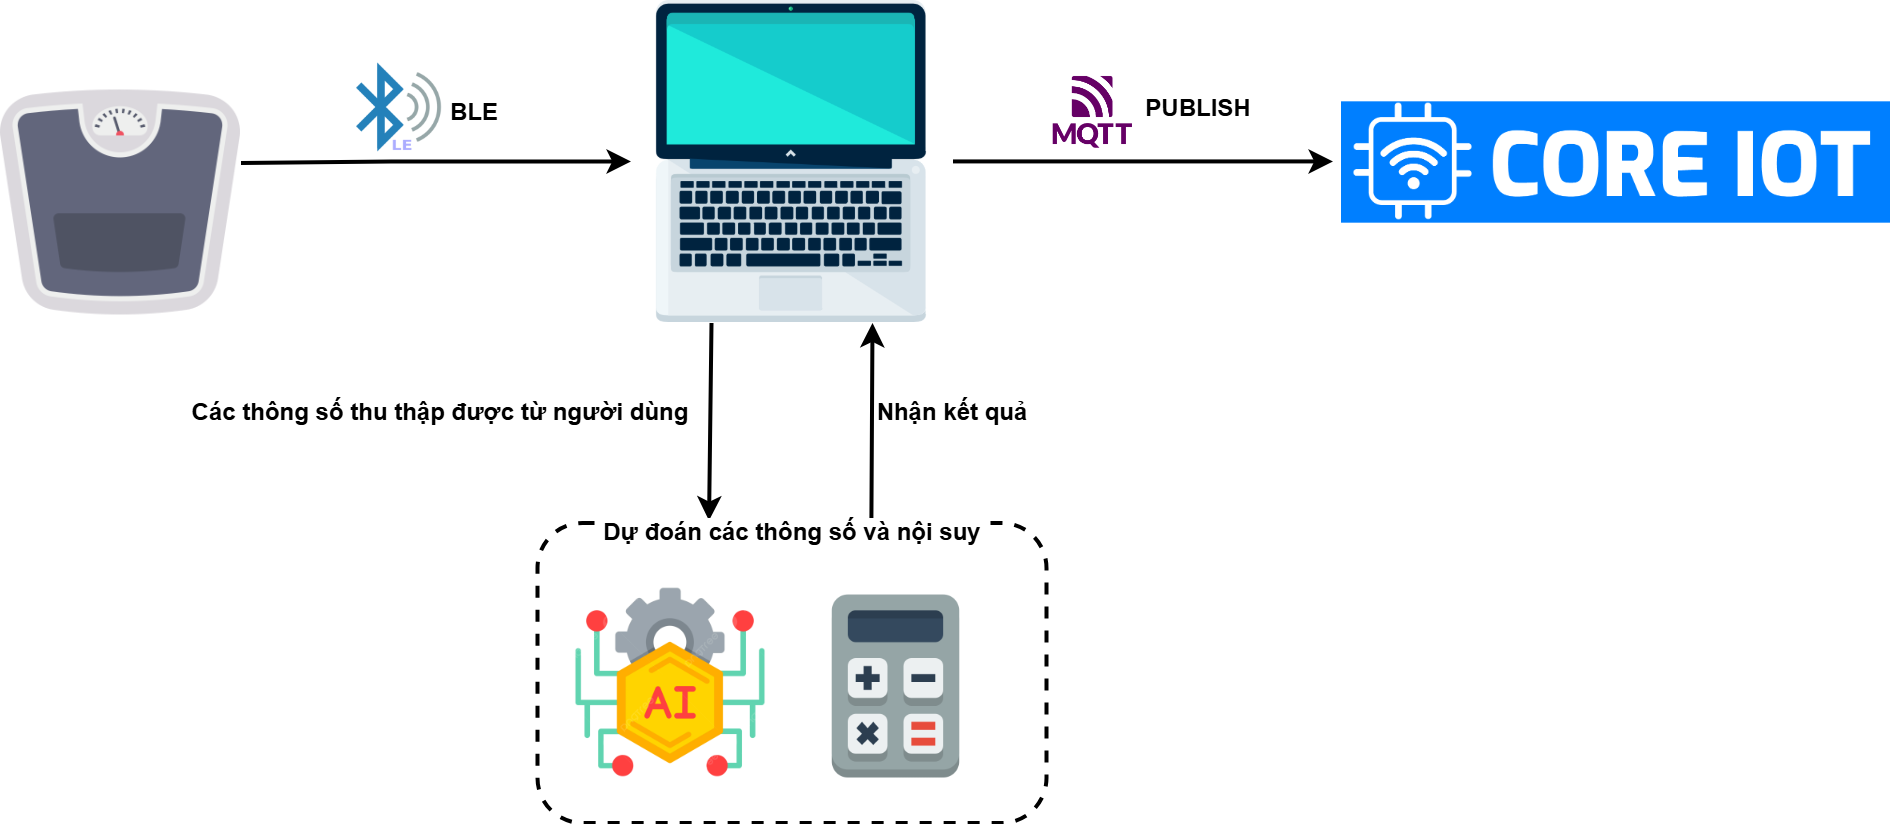
\includegraphics[width=0.9\linewidth]{graphics/scale_diagram.png}
    \caption{Sơ đồ kiến trúc hệ thống chăm sóc sức khỏe điện tử}
\end{figure}

Hình trên minh hoạ luồng dữ liệu và mối quan hệ giữa các thành phần trong hệ thống. Việc áp dụng kiến trúc phân tầng giúp đảm bảo tính mở rộng, dễ bảo trì và hỗ trợ tích hợp thêm các thiết bị mới hoặc dịch vụ y tế số trong tương lai.

\subsection{Thu thập các thông tin cơ bản từ người dùng}
Sử dụng thư viện \href{https://docs.python.org/3/library/tkinter.html}{Tkiner} của Python để tạo hộp thoại yêu cầu người dùng điền 1 số thông tin cá nhân cơ bản để phục vụ cho việc nội suy các chỉ số sức khoẻ.

\begin{figure} [!htp]
    \centering
    
\includegraphics[width=0.6\linewidth]{graphics/hopthoai.jpg}
    \caption{Hộp thoại được tạo bằng thư viện Tkiner để thu thập các thông tin cơ bản của người dùng}
\end{figure}

 Ở hộp thoại này, người dùng có thể nhập mới thông tin, hoặc chọn tên người dùng có sẵn được lưu trữ trước đó trong cơ sở dữ liệu, các thông tin còn lại như ngày sinh, chiều cao, và hệ số hoạt động sẽ được tự động điền.

\subsection{Đọc và phân tích dữ liệu cân nặng từ cân điện tử thông minh}
Đê có thể đọc và phân tích dữ liệu từ cân điện tử thông minh, đầu tiên ta phải biết được UUID của thiết bị. Để làm được điều đó em sử dụng ứng dụng trên điện thoại thông minh có tên "\textbf{BLE Scanner (Connect \& Notify)}" được tải từ CH Play.

\begin{figure} [!htp]
    \centering
    
\includegraphics[width=0.8\linewidth]{graphics/BLE Scanner.png}
    \caption{Ứng dụng BLE Scanner được tải từ CH Play}
\end{figure}

Sử dụng ứng dụng kết nối với 2 thiết bị cân thông  minh \textbf{Xiaomi Smart Scale 2} và \textbf{Crenot Gofit S2} để tìm UUID của 2 thiết bị.

\newpage

\begin{figure} [!htp]
    \centering
    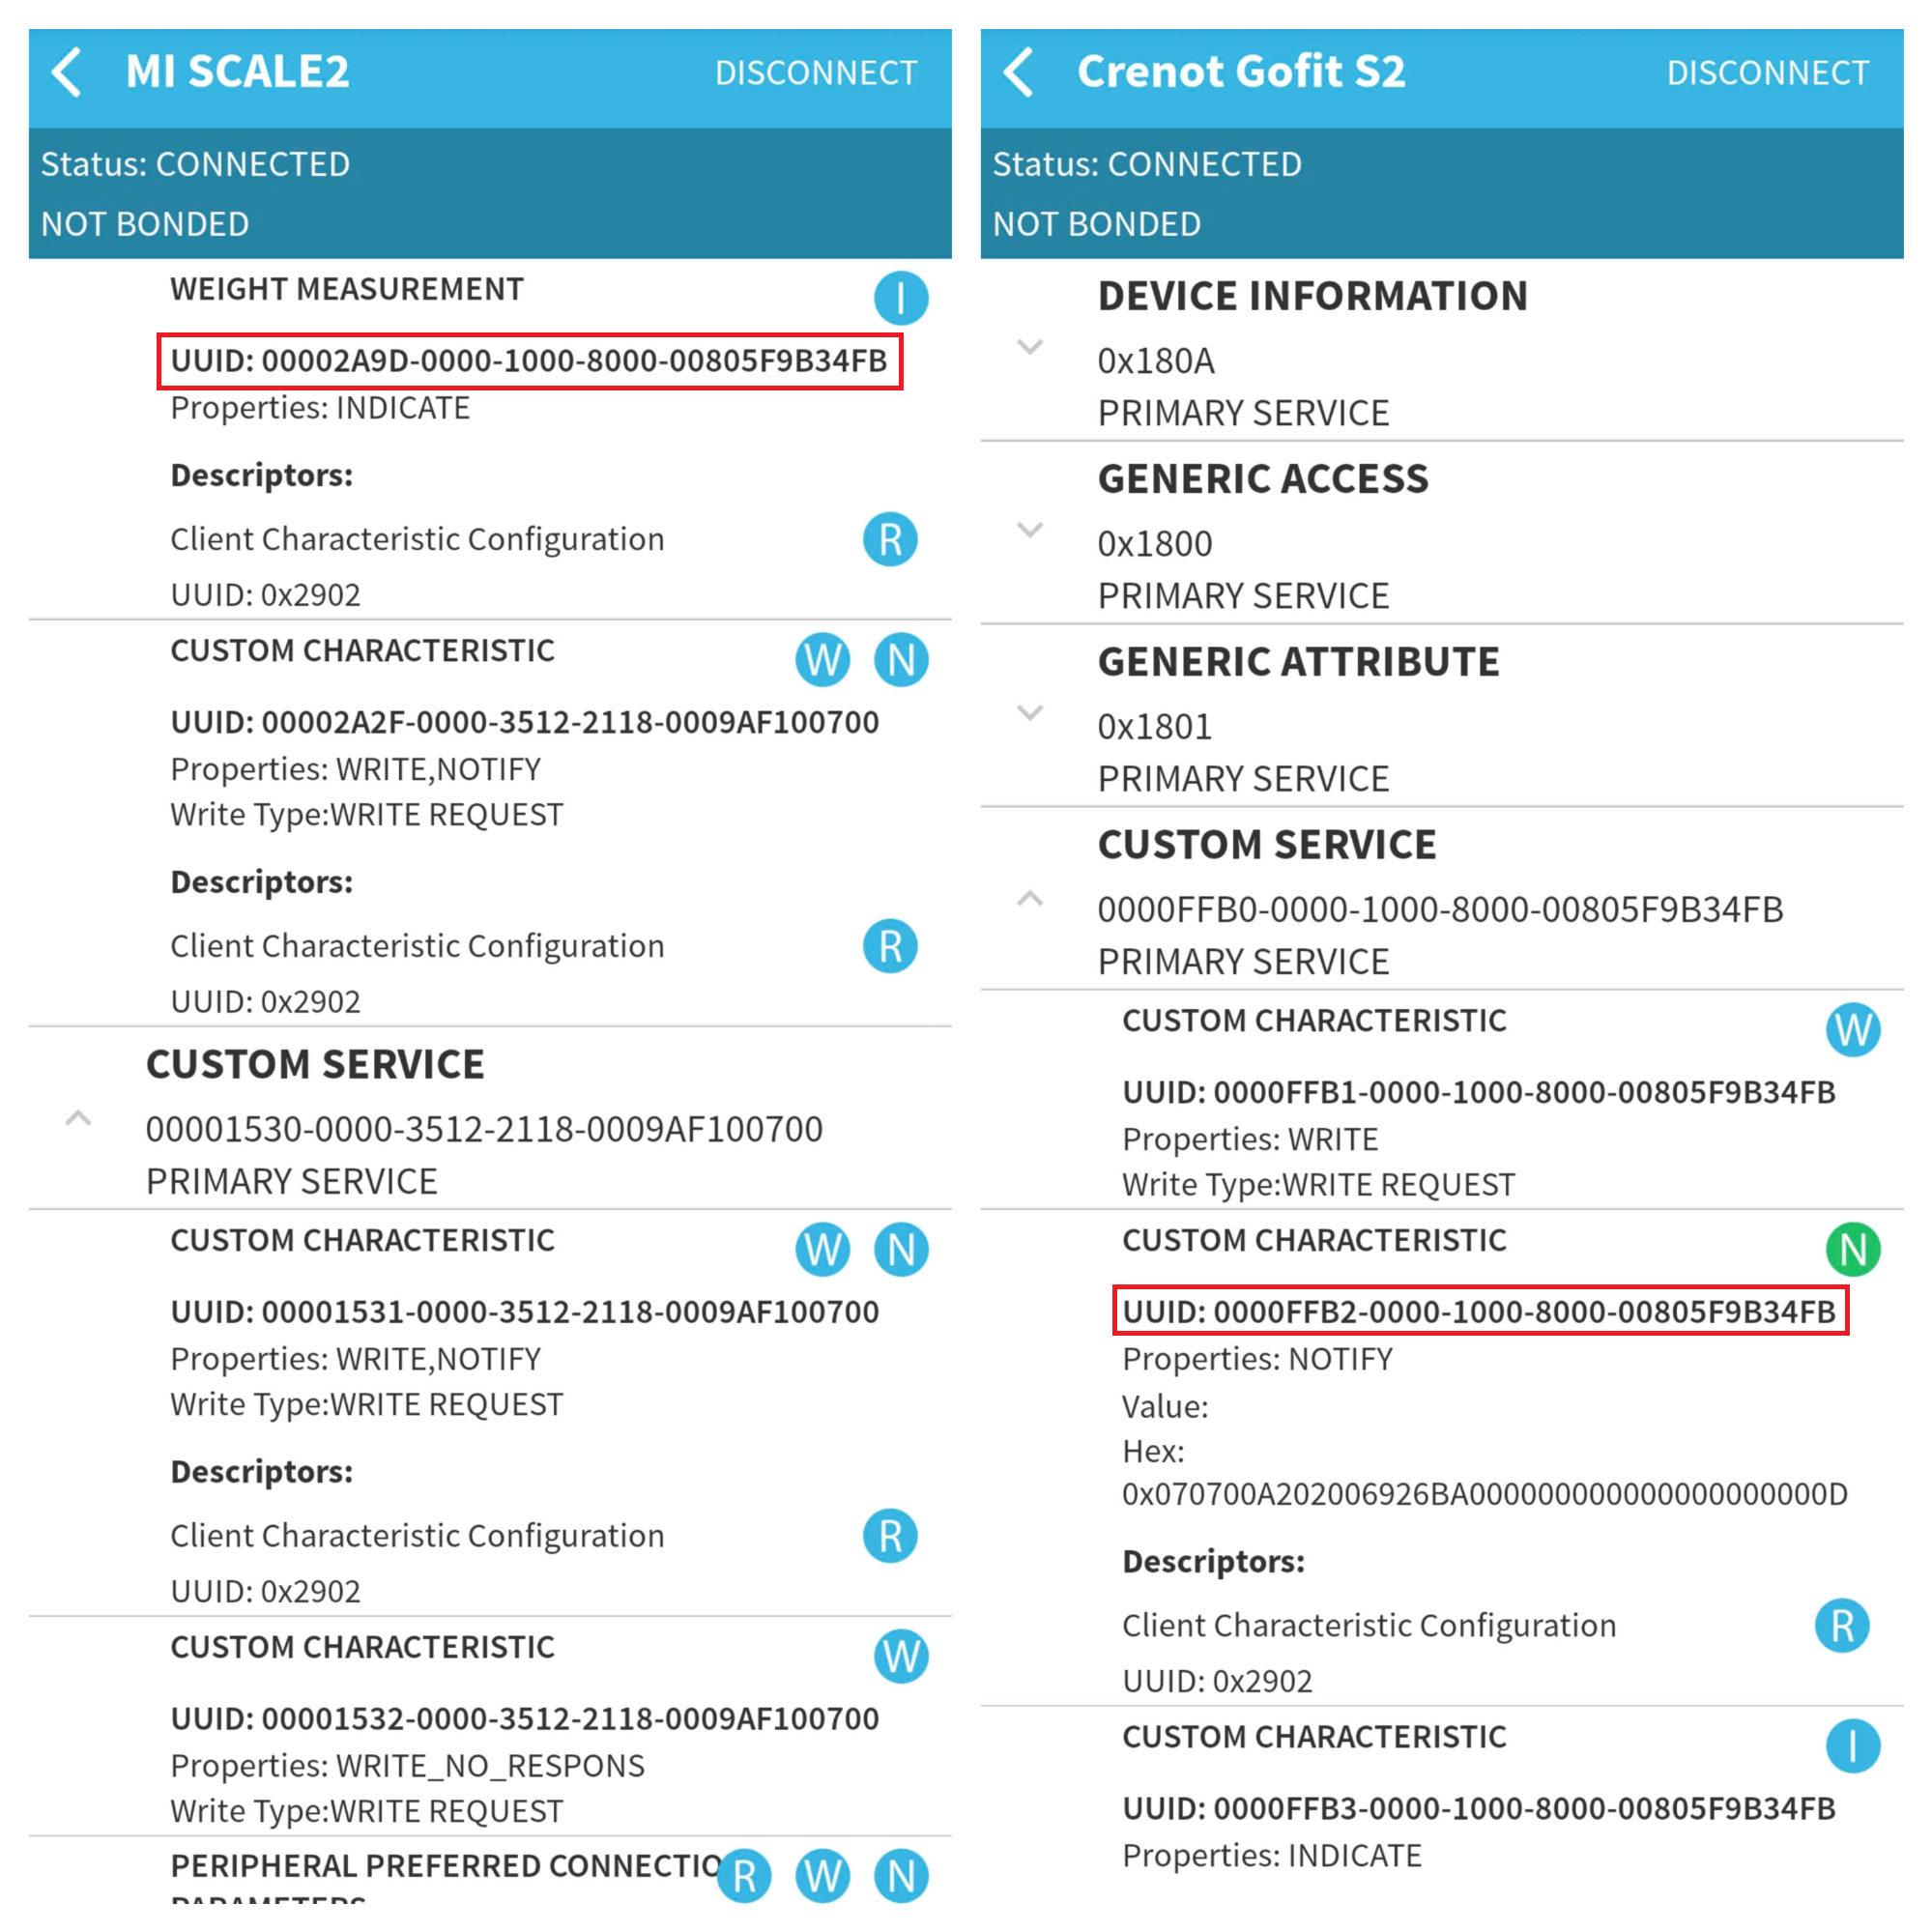
\includegraphics[width=0.6\linewidth]{graphics/miandcrenot.png}
    \caption{Tìm UUID của 2 thiết bị cân điện tử thông minh}
\end{figure}

Ta thu được 2 UUID tương ứng với 2 thiết bị Xiaomi Smart Scale 2 và Crenot Gofit S2 lần lượt như sau:

\begin{itemize}
    \item \textbf{Xiaomi Smart Scale 2 UUID:} 00002A9D-0000-1000-8000-00805F9B34FB
    \item \textbf{Crenot Gofit S2 UUID:} 0000FFB2-0000-1000-8000-00805F9B34FB
\end{itemize}

Sử dụng UUID vừa tìm được để kết nối với thiết bị cân cần nghiên cứu:

\begin{lstlisting}[language=python,caption={Sử dụng UUID để kết nối với thiết bị cần nghiên cứu}]
#DEVICE_NAME = 'MI SCALE2'
#BODY_COMPOSITION_MEASUREMENT_UUID = '00002A9D-0000-1000-8000-00805F9B34FB'  # UUID for the Weight Measurement
# characteristic Mi Scale 2

DEVICE_NAME = 'Crenot Gofit S2'
BODY_COMPOSITION_MEASUREMENT_UUID = '0000FFB2-0000-1000-8000-00805F9B34FB'  # UUID for the Weight Measurement
# characteristic Crenot Gofit S2

async def connect_and_measure():
    disconnected_event = asyncio.Event()

    def disconnected_callback(_bleak_client: BleakClient):
        logger.info("disconnected callback")
        disconnected_event.set()

    device = await find_scale_device()
    if device:
        logger.info(f"found device: {device.name}")
    if not device:
        logger.info("no device found")
        return

    client = BleakClient(device, disconnected_callback = disconnected_callback)

    async with client:
        await client.start_notify(
            BODY_COMPOSITION_MEASUREMENT_UUID, notification_handler
        )
        await disconnected_event.wait()
\end{lstlisting}

\subsubsection{Phân tích dữ liệu được gửi về từ Xiaomi Smart Scale 2}

Sử dụng đoạn code sau để phân tích dữ liệu từ cân Xiaomi ra chỉ số cân nặng có thể đọc được

\begin{lstlisting}[language=python,caption={Code phân tích dữ liệu cân nặng được gửi về từ cân Xiaomi}]
weight = int.from_bytes(data[1:3], byteorder = 'little')/200
\end{lstlisting}

Cụ thể:

\begin{itemize}
    \item data[1:3]: Lấy phần tử thứ 2 và thứ 3 (vì chỉ số bắt đầu từ 0) từ mảng data. Đoạn này là một mảng con chứa hai byte.
    \item int.from\_bytes(..., byteorder='little'): Chuyển đổi hai byte vừa lấy thành một số nguyên, sử dụng thứ tự byte là 'little\-endian' (byte nhỏ nhất nằm ở trước).
    \item / 200: Chia giá trị nguyên đó cho 200 để chuyển đổi thành một giá trị thập phân (theo lý thuyết về dữ liệu được gửi từ thiết bị BLE được trình bày phía trên).
\end{itemize}

\subsubsection{Phân tích dữ liệu được gửi về từ Crenot Gofit S2}

Để tìm được cân nặng được gửi từ thiết bị ta tiến hành khảo sát bằng cách cân thử và đọc dữ liệu gốc (dạng Hex) từ ứng dụng BLE Scanner ta thu được dữ liệu trả về trên ứng dụng như sau:

\begin{itemize}
    \item 76,7 kí: 0XCD0700A202006\textbf{92B9C}000000000000000000001A
    \item 0 kí: 0X3B0700A201006\textbf{80000}000000000000000000000B
\end{itemize}

Nhận thấy dữ liệu gốc trả về tương đồng nhau, chỉ khác nhau ở các phần tử 92B9C (76,6 kí) và 80000 (0 kí). Lấy 2 phần khác nhau trừ nhau ta thu được: 0x92B9C - 0x80000 = 0x12B9C đổi sang hệ DEC ta được 76700. Từ khảo sát trên ta có đoạn code tổng quát để xử lý dữ liệu được gửi về từ cân Crenot Gofit S2 như sau:

\begin{lstlisting}[language=python,caption={Code phân tích dữ liệu cân nặng được gửi về từ cân Crenot Gofit S2}]
weight = round((int(data.hex()[13:18], 16) - 524288) / 1000, 2)
\end{lstlisting}

\subsection{Nội suy các thông số sức khoẻ của cơ thể từ chỉ số cân nặng thu được}
Chỉ số cân nặng thu được từ cân điện tử, có thể được sử dụng để tính toán các thông số sức khoẻ khác của cơ thể dựa theo \href{https://github.com/lolouk44/xiaomi_mi_scale}{các công thức từ ứng dụng Mi Fit của Xiaomi}

\subsubsection{Chỉ số BMI}
Chỉ số BMI (Body Mass Index) là một công cụ được sử dụng để đánh giá mối quan hệ giữa cân nặng và chiều cao của một người, nhằm xác định xem họ có thuộc mức cân nặng bình thường, thừa cân hay thiếu cân hay không. Công thức tính BMI được thực hiện bằng cách lấy cân nặng (kg) chia cho bình phương chiều cao (m). Chỉ số BMI được tính trong project này thông qua hàm như sau:

\begin{lstlisting}[language=python,caption={Hàm tính toán chỉ số BMI của cơ thể}]
def get_bmi(height, weight):
    height_in_meters = height / 100
    return round(weight / (height_in_meters ** 2), 2)
\end{lstlisting}

Ngoài ra, dựa vào chỉ số BMI ta có thể chia ra các tình trạng thể chất như:
\begin{itemize}
    \item BMI < 18.5: Thiếu cân
    \item 18.5 $\leq$ BMI < 24.9: Bình thưởng
    \item 25 $\leq$ BMI < 29.9: Thừa cân
    \item BMI $\geq$ 30: Béo phì
\end{itemize}

\begin{lstlisting}[language=python,caption={Hàm đánh giá chỉ số BMI của cơ thể}]
def evaluate_bmi(bmi, height, weight):
    if bmi < 18.5:
        weight_needed = 18.5 * (height / 100) ** 2 - weight
        # bmi_eval_label.config(fg="blue", font=("Helvetica", 12, "bold"))
        return f"THIEU CAN, BAN CAN TANG KHOANG {weight_needed:.2f} kg."
    elif 18.5 <= bmi < 24.9:
        # bmi_eval_label.config(fg="green", font=("Helvetica", 12, "bold"))
        return "BINH THUONG"
    elif 25 <= bmi < 29.9:
        weight_needed = weight - 24.9 * (height / 100) ** 2
        # bmi_eval_label.config(fg="orange", font=("Helvetica", 12, "bold"))
        return f"THUA CAN, BAN CAN GIAM KHOANG {weight_needed:.2f} kg."
    else:
        weight_needed = weight - 24.9 * (height / 100) ** 2
        # bmi_eval_label.config(fg="red", font=("Helvetica", 12, "bold"))
        return f"BEO PHI. BAN CAN GIAM KHOANG {weight_needed:.2f} kg."
\end{lstlisting}

\subsubsection{Chỉ số TDEE và BMR}
Chỉ số BMR (Basal Metabolic Rate) là lượng calo cơ thể cần để duy trì các chức năng sống cơ bản như hô hấp, tuần hoàn và duy trì nhiệt độ cơ thể khi ở trạng thái nghỉ ngơi hoàn toàn. Đây là yếu tố quan trọng để xác định mức năng lượng tối thiểu cần thiết mỗi ngày.


Chỉ số TDEE (Total Daily Energy Expenditure) là lượng calo mà cơ thể cần để duy trì các hoạt động hàng ngày, bao gồm các hoạt động thể chất và sinh hoạt. TDEE được tính dựa trên BMR và hệ số hoạt động, giúp xác định lượng calo cần thiết để duy trì cân nặng hiện tại hoặc điều chỉnh chế độ ăn uống.

\begin{lstlisting}[language=python,caption={Hàm tính toán chỉ số TDEE và BMR của cơ thể}]
def get_bmr_tdee(weight, height, age, gender, activity_factor):
    if gender == 'male':
        bmr = 88.362 + (13.397 * weight) + (4.799 * height) - (5.677 * age)
    else:
        bmr = 447.593 + (9.247 * weight) + (3.098 * height) - (4.330 * age)
    tdee = bmr * activity_factor
    return round(bmr, 2), round(tdee, 2)
\end{lstlisting}

\subsubsection{Khối lượng cơ thể không mỡ (LBM)}
Chỉ số LBM (Lean Body Mass) hay khối lượng cơ thể không mỡ là một chỉ số thể hiện tổng khối lượng cơ bắp, xương, nước và các mô khác trong cơ thể, không bao gồm mỡ. Đây là một chỉ số quan trọng trong việc đánh giá thành phần cơ thể và theo dõi sức khỏe cũng như hiệu quả của các chương trình tập luyện.

\begin{lstlisting}[language=python,caption={Hàm tính toán chỉ số LBM của cơ thể}]
def get_lbm(height, weight, gender):
    if gender == 'male':
        lbm = (0.32810 * weight) + (0.33929 * height) - 29.5336
        return round(lbm, 2)
    else:
        lbm = (0.29569 * weight) + (0.41813 * height) - 43.2933
        return round(lbm, 2)
\end{lstlisting}

\subsubsection{Tỷ lệ phần trăm nước trong cơ thể}
Đoạn mã dưới đây được thiết kế để tính toán tỷ lệ phần trăm nước trong cơ thể dựa trên các thông tin cá nhân bao gồm giới tính, tuổi, cân nặng và chiều cao. Phương pháp này đóng vai trò quan trọng trong việc đánh giá sức khỏe và thể chất, bởi tỷ lệ nước trong cơ thể ảnh hưởng trực tiếp đến nhiều chức năng sinh lý. Để thực hiện điều này, đoạn mã sử dụng một công thức cơ bản dựa trên tỷ lệ phần trăm mỡ trong cơ thể, sau đó điều chỉnh kết quả bằng một hệ số phù hợp và đảm bảo giá trị cuối cùng nằm trong phạm vi hợp lý về mặt sinh lý học.

Trước tiên, tỷ lệ nước ban đầu được tính toán thông qua công thức sau:
\[
P_{\text{water}} = \left(100 - P_{\text{fat}}(G, A, W, H)\right) \times 0.7
\]
Trong đó, \( P_{\text{fat}}(G, A, W, H) \) biểu thị tỷ lệ phần trăm mỡ trong cơ thể, được xác định dựa trên giới tính (\(G\)), tuổi (\(A\)), cân nặng (\(W\)) và chiều cao (\(H\)) thông qua hàm \texttt{get\_fat\_percentage}. Công thức này xuất phát từ giả định rằng phần không có mỡ của cơ thể (lean body mass) chiếm khoảng 70\% là nước, do đó, sau khi trừ đi tỷ lệ mỡ, phần còn lại được nhân với 0.7 để ước lượng lượng nước.

Tiếp theo, giá trị \( P_{\text{water}} \) được tinh chỉnh bằng một hệ số điều chỉnh (coefficient), phụ thuộc vào mức nước ban đầu:
\[
\text{Coefficient} = 
\begin{cases} 
1.02 & \text{nếu } P_{\text{water}} \leq 50 \\
0.98 & \text{nếu } P_{\text{water}} > 50
\end{cases}
\]
Hệ số này được áp dụng nhằm phản ánh chính xác hơn tỷ lệ nước thực tế, có thể dựa trên các nghiên cứu thực nghiệm hoặc dữ liệu sinh lý. Sau khi xác định hệ số, đoạn mã kiểm tra một điều kiện đặc biệt: nếu \( P_{\text{water}} \times \text{coefficient} \geq 65 \), tỷ lệ nước sẽ được đặt thành 75. Bước này dường như là một cơ chế giới hạn giá trị tối đa, nhằm tránh các kết quả không hợp lý về mặt sinh học. Sau đó, giá trị \( P_{\text{water}} \) được nhân với hệ số và làm tròn đến hai chữ số thập phân để tăng độ chính xác và dễ đọc.

Cuối cùng, kết quả được đưa qua hàm \texttt{check\_val\_overflow} để đảm bảo nằm trong khoảng từ 35 đến 75, một phạm vi được coi là hợp lý về mặt sinh lý học:
\[
P_{\text{water, final}} = \text{CheckValOverflow}(P_{\text{water, adjusted}}, 35, 75)
\]
Hàm này có thể được hiểu là một bước kiểm tra và điều chỉnh, giới hạn giá trị để tránh vượt quá ngưỡng tối thiểu hoặc tối đa cho phép.

Dưới đây là mã nguồn Python minh họa quá trình tính toán:

\begin{lstlisting}[language=python,caption={Hàm tính toán chỉ số phần trăm nước của cơ thể}]
def get_water_percentage(gender, age, weight, height):
    water_percentage = (100 - get_fat_percentage(gender, age, weight, height)) * 0.7

    if water_percentage <= 50:
        coefficient = 1.02
    else:
        coefficient = 0.98

    # Capping water percentage
    if water_percentage * coefficient >= 65:
        water_percentage = 75

    water_percentage = water_percentage * coefficient
    water_percentage = round(water_percentage, 2)

    return check_val_overflow(water_percentage, 35, 75)
\end{lstlisting}

Cụ thể, quá trình triển khai trong mã nguồn bao gồm các bước sau:  
\begin{enumerate}
    \item Tính toán tỷ lệ nước ban đầu bằng cách lấy 100 trừ đi tỷ lệ mỡ (từ hàm \texttt{get\_fat\_percentage}), sau đó nhân với 0.7.  
    \item Xác định hệ số điều chỉnh dựa trên ngưỡng 50 của tỷ lệ nước ban đầu.  
    \item Áp dụng điều kiện giới hạn: nếu tích của tỷ lệ nước và hệ số lớn hơn hoặc bằng 65, giá trị được đặt thành 75.  
    \item Nhân tỷ lệ nước với hệ số và làm tròn kết quả đến hai chữ số thập phân.  
    \item Kiểm tra và điều chỉnh giá trị cuối cùng thông qua hàm \texttt{check\_val\_overflow} để đảm bảo nằm trong khoảng 35 đến 75.
\end{enumerate}

Như vậy, thông qua việc kết hợp công thức toán học và các bước xử lý trong mã nguồn, đoạn mã này cung cấp một phương pháp tính toán tỷ lệ nước trong cơ thể một cách có hệ thống, đồng thời đảm bảo tính chính xác và hợp lý về mặt khoa học.

\subsubsection{Khối lượng xương}

Đoạn mã được thiết kế nhằm tính toán khối lượng xương (\textit{bone mass}) dựa trên các thông tin cá nhân như chiều cao, cân nặng và giới tính. Phương pháp này đóng vai trò quan trọng trong việc đánh giá sức khỏe xương, một yếu tố cốt lõi ảnh hưởng đến sức khỏe tổng thể và khả năng vận động. Để thực hiện, đoạn mã sử dụng một công thức tích hợp giá trị cơ sở khác biệt giữa nam và nữ, kết hợp với khối lượng cơ thể không mỡ (LBM), sau đó tinh chỉnh và giới hạn kết quả để đảm bảo tính hợp lý về mặt sinh lý học.

Trước hết, giá trị cơ sở \( B_{\text{base}} \) được xác định dựa trên giới tính như sau:
\[
B_{\text{base}} = 
\begin{cases} 
0.245691014 & \text{(nữ)} \\
0.18016894 & \text{(nam)}
\end{cases}
\]
Giá trị này phản ánh sự khác biệt sinh học trong cấu trúc xương giữa hai giới. Tiếp theo, khối lượng cơ thể không mỡ (LBM) được tính toán thông qua hàm \texttt{get\_lbm}, dựa trên chiều cao và cân nặng, đại diện cho phần khối lượng cơ thể không bao gồm mỡ, bao gồm cơ bắp, xương và các mô khác.

Sau đó, khối lượng xương ban đầu \( B_{\text{mass}} \) được tính bằng công thức:
\[
B_{\text{mass}} = \left(B_{\text{base}} - (LBM \times 0.05158)\right) \times (-1)
\]
Công thức này suy ra khối lượng xương từ giá trị cơ sở và LBM, với hệ số 0.05158 có thể bắt nguồn từ các nghiên cứu thực nghiệm. Kết quả sau đó được điều chỉnh dựa trên ngưỡng cố định:
\[
B_{\text{mass, adjusted}} = 
\begin{cases} 
B_{\text{mass}} + 0.1 & \text{nếu } B_{\text{mass}} > 2.2 \\
B_{\text{mass}} - 0.1 & \text{nếu } B_{\text{mass}} \leq 2.2
\end{cases}
\]
Bước điều chỉnh này nhằm tinh chỉnh giá trị, đảm bảo phản ánh chính xác hơn các yếu tố sinh lý bổ sung. Tiếp theo, giá trị được giới hạn theo giới tính để tránh các kết quả không thực tế:
\[
B_{\text{mass, capped}} = 
\begin{cases} 
8 & \text{nếu là nữ và } B_{\text{mass, adjusted}} > 5.1 \\
8 & \text{nếu là nam và } B_{\text{mass, adjusted}} > 5.2 \\
B_{\text{mass, adjusted}} & \text{ngược lại}
\end{cases}
\]
Việc áp dụng ngưỡng giới hạn này đảm bảo khối lượng xương phù hợp với đặc điểm sinh lý của từng giới. Cuối cùng, giá trị được kiểm tra và điều chỉnh thông qua hàm \texttt{check\_val\_overflow} để nằm trong khoảng từ 0.5 đến 8:
\[
B_{\text{mass, final}} = \text{CheckValOverflow}(B_{\text{mass, capped}}, 0.5, 8)
\]
Bước này đóng vai trò như một biện pháp kiểm soát cuối cùng, đảm bảo giá trị luôn nằm trong phạm vi hợp lý.

Dưới đây là mã nguồn Python minh họa quá trình tính toán:

\begin{lstlisting}[language=python,caption={Hàm tính toán chỉ số khối lượng xương của cơ thể}]
def get_bone_mass(height, weight, gender):
    if gender == 'female':
        base = 0.245691014
    else:
        base = 0.18016894

    lbm = get_lbm(height, weight, gender)
    bone_mass = (base - (lbm * 0.05158)) * -1

    if bone_mass > 2.2:
        bone_mass += 0.1
    else:
        bone_mass -= 0.1

    # Capping bone_mass
    if gender == 'female' and bone_mass > 5.1:
        bone_mass = 8
    elif gender == 'male' and bone_mass > 5.2:
        bone_mass = 8

    bone_mass = round(bone_mass, 2)

    return check_val_overflow(bone_mass, 0.5, 8)
\end{lstlisting}

\textbf{Giải thích chi tiết}
\begin{itemize}
    \item \( B_{\text{base}} \): Giá trị cơ sở, phụ thuộc vào giới tính, với nữ có giá trị cao hơn nam, phản ánh đặc điểm sinh học.
    \item \( LBM \): Khối lượng cơ thể không mỡ, được tính từ chiều cao và cân nặng qua hàm \texttt{get\_lbm}.
    \item \( B_{\text{mass}} \): Khối lượng xương ban đầu, được suy ra từ \( B_{\text{base}} \) và \( LBM \) theo công thức đã nêu.
    \item \( B_{\text{mass, adjusted}} \): Giá trị sau khi điều chỉnh dựa trên ngưỡng 2.2, tăng hoặc giảm 0.1 tùy trường hợp.
    \item \( B_{\text{mass, capped}} \): Giá trị được giới hạn ở mức tối đa 5.1 (nữ) hoặc 5.2 (nam), nếu vượt quá thì đặt thành 8.
    \item \( B_{\text{mass, final}} \): Giá trị cuối cùng, được kiểm tra bởi hàm \texttt{check\_val\_overflow}, đảm bảo trong khoảng 0.5 đến 8.
\end{itemize}

\subsubsection{Khối lượng cơ bắp}
Đoạn mã được trình bày dưới đây được thiết kế để tính toán khối lượng cơ bắp (\textit{muscle mass}) dựa trên các thông số cá nhân bao gồm giới tính, tuổi, cân nặng và chiều cao. Phương pháp này đóng vai trò quan trọng trong việc đánh giá thành phần cơ thể, đặc biệt là sức mạnh cơ bắp, một yếu tố thiết yếu đối với sức khỏe và hiệu suất vận động. Để đạt được mục tiêu này, đoạn mã áp dụng một công thức trừ đi khối lượng mỡ và khối lượng xương khỏi tổng cân nặng, sau đó tinh chỉnh kết quả bằng cách áp dụng các giới hạn phù hợp với giới tính, đảm bảo giá trị cuối cùng nằm trong phạm vi hợp lý về mặt sinh lý học.

Quá trình tính toán bắt đầu với công thức cơ bản để xác định khối lượng cơ bắp ban đầu:
\[
M_{\text{mass}} = W - \left(\left(P_{\text{fat}}(G, A, W, H) \times 0.01\right) \times W\right) - B_{\text{mass}}(H, W, G)
\]
Trong đó:
\begin{itemize}
    \item \( W \): Cân nặng tổng của cơ thể (kg).
    \item \( P_{\text{fat}}(G, A, W, H) \): Tỷ lệ phần trăm mỡ trong cơ thể, được tính thông qua hàm \texttt{get\_fat\_percentage}, phụ thuộc vào giới tính (\( G \)), tuổi (\( A \)), cân nặng (\( W \)) và chiều cao (\( H \)).
    \item \( B_{\text{mass}}(H, W, G) \): Khối lượng xương, được xác định từ hàm \texttt{get\_bone\_mass} dựa trên chiều cao (\( H \)), cân nặng (\( W \)) và giới tính (\( G \)).
\end{itemize}

Công thức này phản ánh giả định rằng khối lượng cơ bắp là phần còn lại của cân nặng sau khi loại bỏ khối lượng mỡ (tính bằng tỷ lệ phần trăm nhân với cân nặng) và khối lượng xương. Kết quả \( M_{\text{mass}} \) sau đó được điều chỉnh bằng cách áp dụng các giới hạn tối đa dựa trên giới tính:
\[
M_{\text{mass, capped}} = 
\begin{cases} 
120 & \text{nếu là nữ và } M_{\text{mass}} \geq 84 \\
120 & \text{nếu là nam và } M_{\text{mass}} \geq 93.5 \\
M_{\text{mass}} & \text{ngược lại}
\end{cases}
\]
Các ngưỡng 84 (đối với nữ) và 93.5 (đối với nam) được thiết lập để phản ánh giới hạn sinh lý thực tế, trong khi giá trị tối đa 120 được sử dụng để tránh các kết quả không hợp lý. Bước này đảm bảo rằng khối lượng cơ bắp được giới hạn ở mức phù hợp với đặc điểm sinh học của từng giới.

Cuối cùng, giá trị được kiểm tra thông qua hàm \texttt{check\_val\_overflow} để đảm bảo nằm trong khoảng từ 10 đến 120:
\[
M_{\text{mass, final}} = \text{CheckValOverflow}(M_{\text{mass, capped}}, 10, 120)
\]

Hàm này đóng vai trò như một cơ chế kiểm soát, đảm bảo giá trị cuối cùng không vượt quá ngưỡng tối thiểu hoặc tối đa cho phép, từ đó tăng độ tin cậy của kết quả.

Dưới đây là mã nguồn Python minh họa quá trình tính toán:

\begin{lstlisting}[language=python,caption={Hàm tính toán khối lượng cơ bắp của cơ thể}]
def get_muscle_mass(gender, age, weight, height):
    muscle_mass = weight - ((get_fat_percentage(gender, age, weight, height) * 0.01) * weight) - get_bone_mass(height, weight, gender)

    # Capping muscle mass
    if gender == 'female' and muscle_mass >= 84:
        muscle_mass = 120
    elif gender == 'male' and muscle_mass >= 93.5:
        muscle_mass = 120

    muscle_mass = round(muscle_mass, 2)

    return check_val_overflow(muscle_mass, 10, 120)
\end{lstlisting}

\textbf{Giải thích chi tiết}
\begin{itemize}
    \item \( M_{\text{mass}} \): Khối lượng cơ bắp ban đầu, được tính bằng cách trừ khối lượng mỡ (dựa trên tỷ lệ phần trăm mỡ) và khối lượng xương khỏi tổng cân nặng.
    \item \( P_{\text{fat}}(G, A, W, H) \): Tỷ lệ phần trăm mỡ trong cơ thể, được xác định từ hàm \texttt{get\_fat\_percentage}, phản ánh thành phần mỡ dựa trên các thông số cá nhân.
    \item \( B_{\text{mass}}(H, W, G) \): Khối lượng xương, được tính từ hàm \texttt{get\_bone\_mass}, cung cấp giá trị khối lượng xương dựa trên chiều cao, cân nặng và giới tính.
    \item \( M_{\text{mass, capped}} \): Giá trị khối lượng cơ bắp sau khi áp dụng giới hạn tối đa, với ngưỡng 84 (nữ) hoặc 93.5 (nam), và giá trị tối đa được đặt thành 120.
    \item \( M_{\text{mass, final}} \): Giá trị cuối cùng, được kiểm tra bởi hàm \texttt{check\_val\_overflow}, đảm bảo nằm trong khoảng 10 đến 120, phù hợp với các giới hạn sinh lý.
\end{itemize}

\subsubsection{Tỷ lệ phần trăm đạm của cơ thể}
Đoạn mã dưới đây được thiết kế nhằm tính toán tỷ lệ phần trăm protein trong cơ thể, một chỉ số quan trọng để đánh giá thành phần cơ thể và tình trạng sức khỏe tổng thể. Phương pháp tính toán này dựa trên các thông số cá nhân bao gồm giới tính, tuổi, cân nặng và chiều cao. Người dùng có thể lựa chọn giữa hai phương pháp: phương pháp gốc (\texttt{orig=True}) và phương pháp thay thế (\texttt{orig=False}). Kết quả cuối cùng được tinh chỉnh để đảm bảo nằm trong khoảng giá trị hợp lý về mặt sinh lý học.

\textbf{Phương pháp gốc (\texttt{orig=True})}

Phương pháp này sử dụng khối lượng cơ bắp và tỷ lệ nước trong cơ thể để suy ra tỷ lệ protein. Công thức áp dụng được biểu diễn như sau:
\[
P_{\text{protein}} = \left( \frac{M_{\text{mass}}(G, A, W, H)}{W} \right) \times 100 - P_{\text{water}}(G, A, W, H)
\]
Trong đó:
\begin{itemize}
    \item \( M_{\text{mass}}(G, A, W, H) \): Khối lượng cơ bắp, được tính dựa trên giới tính (\( G \)), tuổi (\( A \)), cân nặng (\( W \)) và chiều cao (\( H \)).
    \item \( W \): Cân nặng tổng của cơ thể, đơn vị là kilogam.
    \item \( P_{\text{water}}(G, A, W, H) \): Tỷ lệ phần trăm nước trong cơ thể, được xác định thông qua hàm phù hợp.
\end{itemize}

Phương pháp này dựa trên giả định rằng protein chiếm phần lớn trong cơ bắp sau khi loại bỏ thành phần nước, từ đó tính toán tỷ lệ protein bằng cách lấy tỷ lệ cơ bắp trừ đi tỷ lệ nước.

\textbf{Phương pháp thay thế (\texttt{orig=False})}

Ngược lại, phương pháp thay thế tính toán tỷ lệ protein bằng cách loại bỏ các thành phần khác của cơ thể (bao gồm mỡ, nước và xương) khỏi tổng 100\%. Công thức cụ thể được thể hiện như sau:

\begin{align*}
P_{\text{protein}} &= 100 - \left\lfloor P_{\text{fat}}(G, A, W, H) \times 100 \right\rfloor / 100 \\
&\quad - \left\lfloor P_{\text{water}}(G, A, W, H) \times 100 \right\rfloor / 100 \\
&\quad - \left\lfloor \frac{B_{\text{mass}}(H, W, G)}{W} \times 100 \times 100 \right\rfloor / 100
\end{align*}

Trong đó:
\begin{itemize}
    \item \( P_{\text{fat}}(G, A, W, H) \): Tỷ lệ phần trăm mỡ trong cơ thể, được xác định từ hàm tương ứng.
    \item \( B_{\text{mass}}(H, W, G) \): Khối lượng xương, được tính dựa trên chiều cao, cân nặng và giới tính.
    \item \( \left\lfloor x \times 100 \right\rfloor / 100 \): Thao tác làm tròn giá trị \( x \) đến hai chữ số thập phân để đảm bảo độ chính xác.
\end{itemize}

Phương pháp này xem protein như phần còn lại sau khi đã trừ đi các thành phần chính khác của cơ thể, mang lại một cách tiếp cận toàn diện hơn.

\textbf{Kết quả cuối cùng}

Sau khi áp dụng một trong hai phương pháp trên, tỷ lệ protein được làm tròn đến hai chữ số thập phân và kiểm tra để đảm bảo nằm trong khoảng từ 5 đến 32, thông qua công thức:
\[
P_{\text{protein, final}} = \text{CheckValOverflow}(P_{\text{protein}}, 5, 32)
\]
Bước kiểm tra này đóng vai trò như một biện pháp bảo vệ, đảm bảo kết quả không vượt quá ngưỡng sinh lý hợp lý, từ đó tăng tính tin cậy của phép tính.

\textbf{Mã nguồn minh họa}

Dưới đây là đoạn mã Python thể hiện quá trình tính toán tỷ lệ protein trong cơ thể:

\begin{lstlisting}[language=python,caption={Hàm tính toán chỉ số phần trăm đạm của cơ thể}]
def get_protein_percentage(gender, age, weight, height, orig=True):
    # Use the original algorithm from mi fit (or legacy guess one)
    if orig:
        protein_percentage = (get_muscle_mass(gender, age, weight, height) / weight) * 100
        protein_percentage -= get_water_percentage(gender, age, weight, height)
    else:
        protein_percentage = 100 - (floor(get_fat_percentage(gender, age, weight, height) * 100) / 100)
        protein_percentage -= floor(get_water_percentage(gender, age, weight, height) * 100) / 100
        protein_percentage -= floor((get_bone_mass(height, weight, gender) / weight * 100) * 100) / 100

    protein_percentage = round(protein_percentage, 2)

    return check_val_overflow(protein_percentage, 5, 32)
\end{lstlisting}

\textbf{Giải thích chi tiết các ký hiệu}

\begin{itemize}
    \item \( P_{\text{protein}} \): Tỷ lệ phần trăm protein trong cơ thể, là mục tiêu chính của phép tính.
    \item \( M_{\text{mass}}(G, A, W, H) \): Khối lượng cơ bắp, được sử dụng trong phương pháp gốc.
    \item \( P_{\text{water}}(G, A, W, H) \): Tỷ lệ phần trăm nước, thành phần quan trọng trong cả hai phương pháp.
    \item \( P_{\text{fat}}(G, A, W, H) \): Tỷ lệ phần trăm mỡ, được sử dụng trong phương pháp thay thế.
    \item \( B_{\text{mass}}(H, W, G) \): Khối lượng xương, yếu tố bổ sung trong phương pháp thay thế.
    \item \( \left\lfloor x \times 100 \right\rfloor / 100 \): Thao tác làm tròn nhằm duy trì độ chính xác của kết quả.
    \item \( \text{CheckValOverflow}(x, \text{min}, \text{max}) \): Hàm kiểm tra và giới hạn giá trị \( x \) trong khoảng từ 5 đến 32, phù hợp với thực tế sinh lý.
\end{itemize}

\subsubsection{Mỡ nội tạng}

Phần mã này được thiết kế để ước tính lượng mỡ nội tạng (\emph{visceral fat}) dựa trên hai điều kiện so sánh giữa chiều cao và cân nặng, cùng với tuổi. Mỡ nội tạng thường tập trung quanh vùng bụng, ảnh hưởng đến sức khỏe tim mạch và chuyển hóa. Do đó, việc tính toán chính xác giúp theo dõi và cải thiện tình trạng sức khỏe. Phương pháp tính toán bao gồm hai trường hợp, sau khi xác định đúng công thức sẽ làm tròn và kiểm soát kết quả trong ngưỡng hợp lý từ 1 đến 50.

\textbf{Trường hợp \(H < W \times 1.6\)}
\begin{itemize}
    \item Tính giá trị trung gian:
    \[
      \text{sub\_calc} = \bigl(H \times 0.4 - H \times (H \times 0.0826)\bigr)\times(-1)
    \]
    \item Tính lượng mỡ nội tạng:
    \[
      V_{\text{fat}} = \frac{W \times 305}{\text{sub\_calc} + 48} - 2.9 + (A \times 0.15)
    \]
\end{itemize}

\textbf{Trường hợp ngược lại}
\begin{itemize}
    \item Tính giá trị trung gian:
    \[
      \text{sub\_calc} = 0.765 + H \times (-0.0015)
    \]
    \item Tính lượng mỡ nội tạng:
    \[
      V_{\text{fat}} = \bigl(H \times 0.143 - W \times \text{sub\_calc}\bigr)\times(-1) + (A \times 0.15) - 5.0
    \]
\end{itemize}

\textbf{Xử lý kết quả cuối cùng}

Sau khi chọn công thức phù hợp, giá trị \(V_{\text{fat}}\) được làm tròn đến hai chữ số thập phân và đảm bảo nằm trong khoảng từ 1 đến 50:
\[
  V_{\text{fat, final}} = \text{CheckValOverflow}\bigl(\,\text{round}(V_{\text{fat}},2),\,1,\,50\bigr)
\]

\textbf{Ý nghĩa các biến số}
\begin{itemize}
  \item \(H\): chiều cao (m)  
  \item \(W\): cân nặng (kg)  
  \item \(A\): tuổi (năm)  
  \item \(\text{sub\_calc}\): giá trị trung gian phục vụ công thức  
  \item \(V_{\text{fat}}\): lượng mỡ nội tạng trước khi kiểm soát  
  \item \(\text{CheckValOverflow}(x,\min,\max)\): hàm giới hạn giá trị \(x\) trong \([\min,\max]\)
\end{itemize}

\textbf{Mã nguồn minh họa}

\begin{lstlisting}[language=python,caption={Hàm tính chỉ số mỡ nội tạng}]
def get_visceral_fat(height, weight, age):
    if height < weight * 1.6:
        sub_calc = ((height * 0.4) - (height * (height * 0.0826))) * -1
        visceral_fat = ((weight * 305) / (sub_calc + 48)) - 2.9 + (age * 0.15)
    else:
        sub_calc = 0.765 + height * -0.0015
        visceral_fat = (((height * 0.143) - (weight * sub_calc)) * -1) + (age * 0.15) - 5.0

    visceral_fat = round(visceral_fat, 2)
    return check_val_overflow(visceral_fat, 1, 50)
\end{lstlisting}

\subsubsection{Căn nặng lý tưởng}

Phần mã này được thiết kế để ước tính trọng lượng lý tưởng (\textit{ideal weight}) dựa trên các thông số cá nhân bao gồm giới tính và chiều cao. Trọng lượng lý tưởng đóng vai trò quan trọng trong việc đánh giá tình trạng sức khỏe tổng thể và là cơ sở để xác định các mục tiêu về cân nặng. Phương pháp tính toán được điều chỉnh linh hoạt, cho phép người dùng lựa chọn giữa hai cách tiếp cận: phương pháp gốc (\texttt{orig=True}) và phương pháp thay thế (\texttt{orig=False}). Kết quả cuối cùng được giới hạn trong khoảng từ 5.5 đến 198 để đảm bảo tính hợp lý.

\textbf{Công thức dành cho phương pháp gốc (\texttt{orig=True})}

Phương pháp này sử dụng các hệ số chuẩn khác nhau cho nữ và nam, phản ánh sự khác biệt sinh học giữa hai giới:

\begin{itemize}
    \item Với giới tính nữ:
    \[
    W_{\text{ideal}} = (H - 70) \times 0.6
    \]
    \item Với giới tính nam:
    \[
    W_{\text{ideal}} = (H - 80) \times 0.7
    \]
\end{itemize}

Trong đó, \( H \) là chiều cao tính bằng centimet. Công thức này dựa trên giả định rằng trọng lượng lý tưởng tỷ lệ thuận với phần chiều cao vượt quá một ngưỡng nhất định (70 cm cho nữ và 80 cm cho nam), với các hệ số điều chỉnh khác nhau cho từng giới.

\textbf{Công thức dành cho phương pháp thay thế (\texttt{orig=False})}

Phương pháp này sử dụng chỉ số BMI (\textit{Body Mass Index}) chuẩn để tính toán trọng lượng lý tưởng:
\[
W_{\text{ideal}} = \frac{22 \times H^2}{10000}
\]

Trong đó, \( H \) là chiều cao tính bằng centimet. Công thức này xuất phát từ việc áp dụng giá trị BMI lý tưởng là 22, một con số thường được coi là khỏe mạnh cho người trưởng thành. Bằng cách sử dụng công thức BMI đảo ngược, trọng lượng lý tưởng được tính toán dựa trên chiều cao và giá trị BMI mong muốn.

\textbf{Xử lý kết quả cuối cùng}

Sau khi áp dụng công thức phù hợp, giá trị \( W_{\text{ideal}} \) được làm tròn đến hai chữ số thập phân. Đối với phương pháp thay thế, kết quả còn được kiểm tra để đảm bảo nằm trong khoảng từ 5.5 đến 198 thông qua hàm:
\[
W_{\text{ideal, final}} = \text{CheckValOverflow}(W_{\text{ideal}}, 5.5, 198)
\]
Bước này giúp giới hạn kết quả trong ngưỡng hợp lý, tránh các giá trị không thực tế hoặc không phù hợp với bối cảnh sinh lý.

\textbf{Ý nghĩa các biến số}

\begin{itemize}
    \item \( W_{\text{ideal}} \): Trọng lượng lý tưởng, tính bằng kilogam.
    \item \( H \): Chiều cao, tính bằng centimet.
    \item \( \text{CheckValOverflow}(x, \text{min}, \text{max}) \): Hàm kiểm soát giá trị \( x \), đảm bảo không vượt quá khoảng từ 5.5 đến 198.
\end{itemize}

\textbf{Mã nguồn minh họa}

Dưới đây là đoạn mã Python triển khai quá trình tính toán trọng lượng lý tưởng:

\begin{lstlisting}[language=python,caption={Hàm tính toán cân nặng lý tưởng của cơ thể}]
def get_ideal_weight(gender, height, orig=True):
    # Uses mi fit algorithm (or Holtek's one)
    if orig and gender == 'female':
        ideal_weight = (height - 70) * 0.6
        return round(ideal_weight, 2)
    elif orig and gender == 'male':
        ideal_weight = (height - 80) * 0.7
        return round(ideal_weight, 2)
    else:
        ideal_weight = (22 * height) * height / 10000
        ideal_weight = round(ideal_weight, 2)
        return check_val_overflow(ideal_weight, 5.5, 198)
\end{lstlisting}

\subsection{Các tính năng liên quan đến trí tuệ nhân tạo và thị giác máy tính}
\subsubsection{Dự đoán giới tính của người dùng thông qua cân nặng và chiều cao}
Để có thể dự đoán được giới tính người dùng thông qua 2 thông số cân nặng và chiều cao, cần chọn 1 bộ dữ liệu phù hợp cho quá trình huấn luyện để có kết quả tối ưu. Cụ thể, bộ dữ liệu được chọn  gồm 3 đặc tính \textbf{"Gender"}, \textbf{"Height"}, và \textbf{"Weight"}, với số lượng 10000 mẫu:

\begin{table}[!htp]
\centering
\begin{tabular}{l|r|r|}
\cline{2-3}
                            & \textbf{Height}       & \textbf{Weight}       \\ \hline
\multicolumn{1}{|l|}{count} & 10000.000000 & 10000.000000 \\ \hline
\multicolumn{1}{|l|}{mean}  & 168.573602   & 73.228114    \\ \hline
\multicolumn{1}{|l|}{std}   & 9.772721     & 14.564143    \\ \hline
\multicolumn{1}{|l|}{min}   & 137.828359   & 29.347484    \\ \hline
\multicolumn{1}{|l|}{25\%}  & 161.304276   & 61.606032    \\ \hline
\multicolumn{1}{|l|}{50\%}  & 168.447898   & 73.124954    \\ \hline
\multicolumn{1}{|l|}{75\%}  & 175.702625   & 84.898668    \\ \hline
\multicolumn{1}{|l|}{max}   & 200.656806   & 122.465267   \\ \hline
\end{tabular}
\caption{Đặc tính của bộ dữ liệu dùng để huấn luyện}
\end{table}

Dựa vào những thông tin trên, nhận xét về bộ dữ liệu như sau
\begin{itemize}
    \item \textbf{Trung bình:} Một người trung bình trong mẫu dữ liệu có chiều cao là 168.57 cm và cân nặng là 73.23 kg.
    \item \textbf{Giá trị nhỏ nhất và lớn nhất:} Chiều cao thấp nhất của người trong mẫu là 137.83 cm, trong khi chiều cao lớn nhất là 200.66 cm. Người nhẹ nhất trong mẫu cân nặng 29.35 kg và người nặng nhất là 122.47 kg.
    \item \textbf{Phân vị:} 25\% số người trong mẫu có chiều cao dưới 161.30 cm, trong khi 25\% số người có chiều cao trên 175.70 cm. 25\% số người trong mẫu có cân nặng dưới 61.61 kg, trong khi 25\% số người có cân nặng trên 84.90 kg.
    \item \textbf{Trung vị:} 50\% số người trong mẫu có chiều cao khoảng 168.45 cm. 50\% số người trong mẫu có cân nặng khoảng 73.12 kg.
    \item \textbf{Độ lệch chuẩn:} Trung bình, chiều cao của một người thay đổi 9.77 cm so với chiều cao trung bình. Trung bình, cân nặng của một người thay đổi 14.56 kg so với cân nặng trung bình.
\end{itemize}

Vì đây là bài toán phân loại nhị phân nên cân nhắc lựa chọn các mô hình phân loại sau:
\begin{enumerate}
    \item Binary Decision Tree
    \item Support Vector Machine
    \item k-n Neighbours Classifier
    \item Naive Bayes Classifier
\end{enumerate}

Đánh giá độ chính xác của từng mô hình phân loại trên bộ dữ liệu được chọn ta có kết quả như sau:

\begin{figure}[!htp]
    \centering
    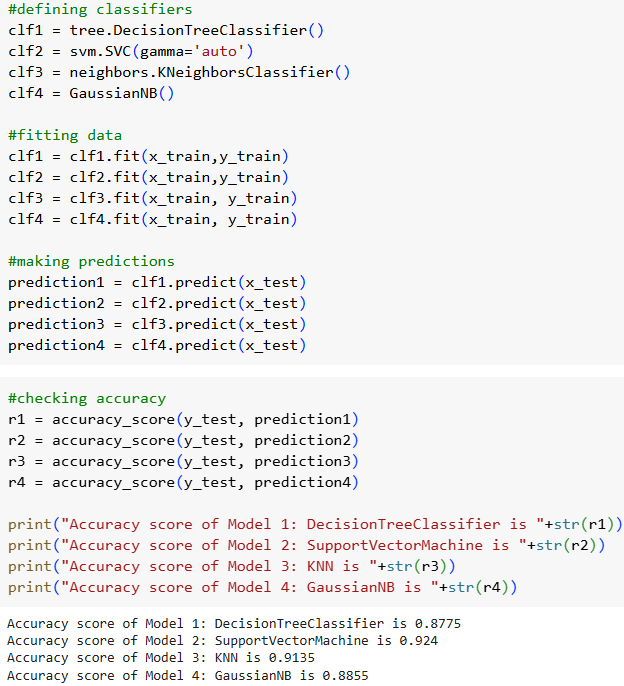
\includegraphics[width=0.8\linewidth]{graphics/dochinhxac.png}
    \caption{Độ chính xác của từng phân loại trên tập dữ liệu được chọn}
\end{figure}

\newpage

Nhìn chung, độ chính xác của phân loại Support Vector Machine cao nhất trong tất cả các phân loại (92,4\%)

Tiếp theo, cần phải có đánh giá về tỷ lệ phân loại sai của các mô hình phân loại:

\begin{figure} [!htp]
    \centering
    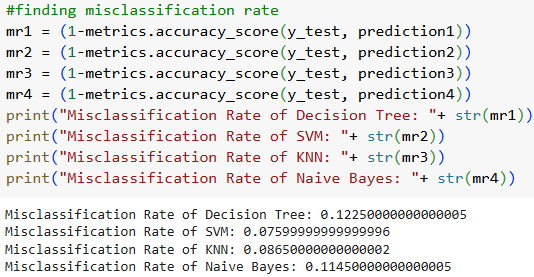
\includegraphics[width=0.75\linewidth]{graphics/sai.png}
    \caption{Tỷ lệ phân loại sai của từng mô hình phân loại trên tập dữ liệu được chọn}
\end{figure}

Vậy mô hình phân loại Support Vector Machine có tỷ lệ phân loại sai thấp nhất (7,6\%). Nên lựa chọn mô hình phân loại Support Vector Machine cho bài toán dự đoán giới tính là phù hợp nhất.

Lưu lại các tham số đã huấn luyện của mô hình trước đó và tiến hành chạy thử với dữ liệu giả định \textbf{chiều cao 166cm} và \textbf{cân nặng 77.7} kí ta thu được kết quả như sau:

\begin{figure}[!htp]
    \centering
    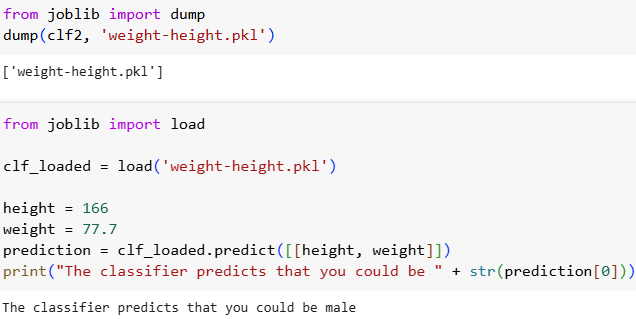
\includegraphics[width=0.75\linewidth]{graphics/ketqua_gender.png}
    \caption{Kết quả khi sử dụng mô hình SVM để dự đoán giới tính thông qua chiều cao và cân nặng}
\end{figure}

\subsubsection{Dự đoán tỷ lệ phần trăm mỡ của cơ thể}
Mặc dù trên ứng dụng Mi Fit có công thức tính toán tỷ lệ phần trăm mỡ của cơ thể, tuy nhiên sai số khi đo với cảm biến là rất lớn. Nhằm để giảm chi phí lắp đặt cảm biến lên cân cũng như giảm diện tích của trạm cân sức khoẻ nên em sử dụng trí tuệ nhân tạo (AI) để dự đoán cân nặng của 1 người thông qua các thông số như: độ tuổi, giới tính, chiều cao, và cân nặng. Mô hình được huấn luyện trên tập dữ liệu gồm các thông số như: \textbf{age}, \textbf{gender}, \textbf{height\_cm}, \textbf{weight\_kg}, \textbf{body\_fat}, \textbf{diastolic}, \textbf{systolic}, \textbf{gripForce}, \textbf{sit and bend forward\_cm}, \textbf{sit-ups counts}, \textbf{broad jump\_cm}, và \textbf{class} và khoảng 13400 bảng ghi. Cụ thể thông tin về bộ dữ liệu như sau:

\begin{figure} [!htp]
    \centering
    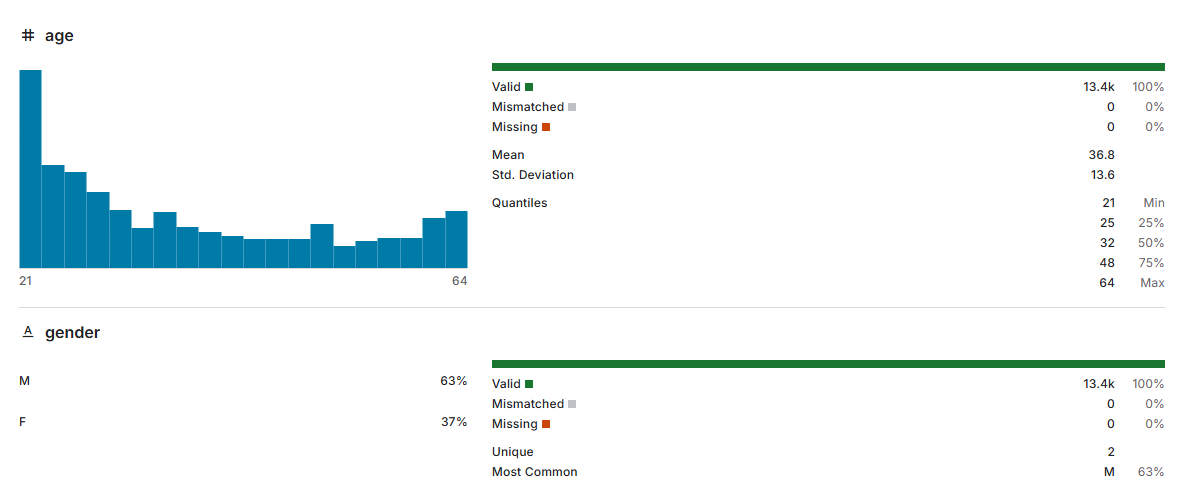
\includegraphics[width=1\linewidth]{graphics/BP_dataset_dotuoi_gioitinh.png}
    \caption{Thông tin độ tuổi và giới tính có trong bộ dữ liệu được huấn luyện để dự đoán tỷ lệ phần trăm mỡ trong cơ thể}
\end{figure}

\newpage

\begin{figure} [!htp]
    \centering
    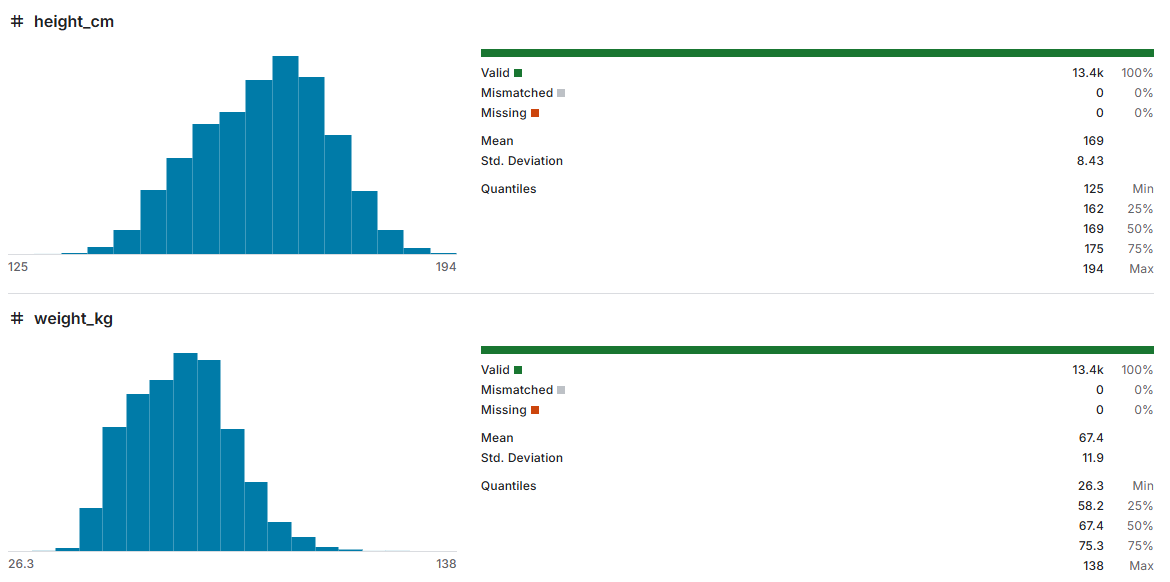
\includegraphics[width=1\linewidth]{graphics/BP_dataset_chieucao_cannang.png}
    \caption{Thông tin chiều cao và cân nặng có trong bộ dữ liệu được huấn luyện để dự đoán tỷ lệ phần trăm mỡ trong cơ thể}
\end{figure}

\begin{figure} [!htp]
    \centering
    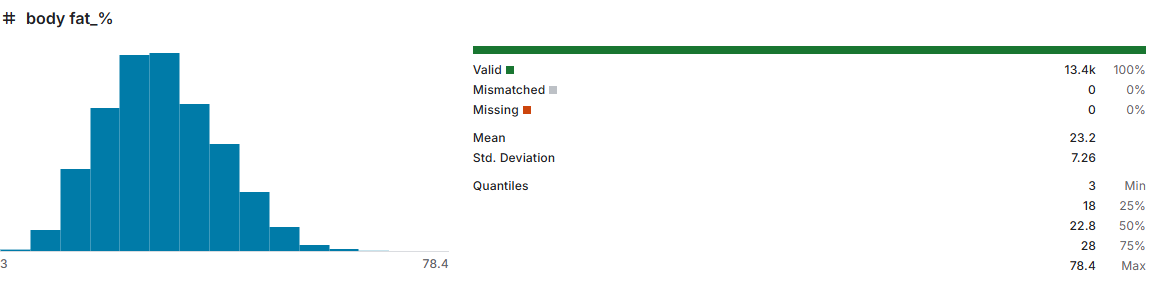
\includegraphics[width=1\linewidth]{graphics/BP_dataset_tylemo.png}
    \caption{Thông tin về tỷ lệ mỡ có trong bộ dữ liệu được huấn luyện để dự đoán tỷ lệ phần trăm mỡ trong cơ thể}
\end{figure}

Do bộ dữ liệu là dữ liệu liên tục (tuổi, chiều cao, cân nặng, tỷ lệ mỡ cơ thể). Hồi quy tuyến tính hoạt động tốt với các loại dữ liệu này, giúp xây dựng một đường thẳng để dự đoán giá trị liên tục của biến phụ thuộc dựa trên các biến độc lập. Nên chọn mô hình Hồi quy tuyến tính \textbf{(Linear Regression model)} là phù hợp để giải quyết bài toán dự đoán tỷ lệ mỡ của cơ thể. Sau khi sử dụng mô hình hồi quy tuyến tính trên bộ dữ liệu để dự đoán tỷ lệ mỡ em thu được các kết quả như sau:

\newpage

\begin{figure} [!htp]
    \centering
    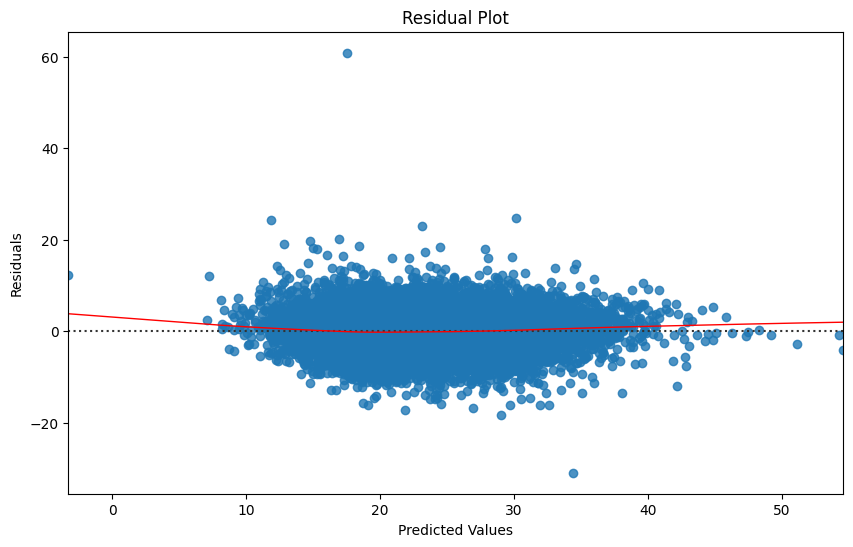
\includegraphics[width=0.8\linewidth]{graphics/residual_plot.png}
    \caption{Biểu đồ phần dư}
\end{figure}

Biểu đồ phần dư được sử dụng để kiểm tra độ phù hợp của mô hình hồi quy. Trên trục hoành là các giá trị dự đoán, còn trục tung biểu diễn phần dư (sai số giữa giá trị thực tế và giá trị dự đoán).

Một phân bố ngẫu nhiên của phần dư xung quanh trục 0 cho thấy mô hình phù hợp với dữ liệu và các giả định về tuyến tính và phương sai không đổi của sai số được đáp ứng.

Trong biểu đồ này, phần dư không có xu hướng rõ ràng theo bất kỳ hướng nào, tuy nhiên, có một số điểm ngoại lệ rõ rệt ở phía trên và dưới. Điều này cho thấy rằng, nhìn chung, mô hình có thể phù hợp, nhưng có thể cần xem xét lại các ngoại lệ đó để cải thiện chất lượng dự đoán hoặc xác minh các giả định.

\newpage

\begin{figure} [!htp]
    \centering
    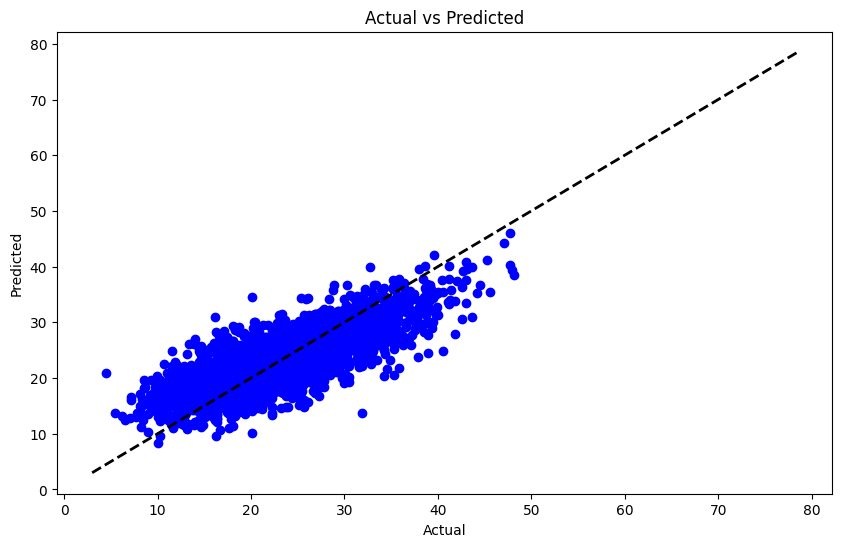
\includegraphics[width=0.8\linewidth]{graphics/ac_vs_pre.png}
    \caption{Biểu đồ phân tán}
\end{figure}

\textbf{Mối quan hệ tuyến tính:} Các điểm dữ liệu có xu hướng phân bố theo một đường thẳng, cho thấy có mối quan hệ tuyến tính giữa giá trị dự đoán và giá trị thực tế.

\textbf{Độ chính xác:} Phần lớn các điểm dữ liệu nằm gần đường thẳng y=x, cho thấy mô hình dự đoán khá chính xác. Tuy nhiên, vẫn có một số điểm dữ liệu nằm xa đường thẳng này, đặc biệt ở vùng giá trị lớn hơn 60.

\textbf{Các điểm ngoại lệ:} Có một số điểm dữ liệu nằm khá xa các điểm khác, đặc biệt ở vùng giá trị lớn hơn 60.

Biểu đồ phân tán này cho thấy mô hình dự đoán đã xây dựng được một mối quan hệ tuyến tính khá tốt giữa các biến độc lập và biến phụ thuộc.

\newpage

\begin{figure} [!htp]
    \centering
    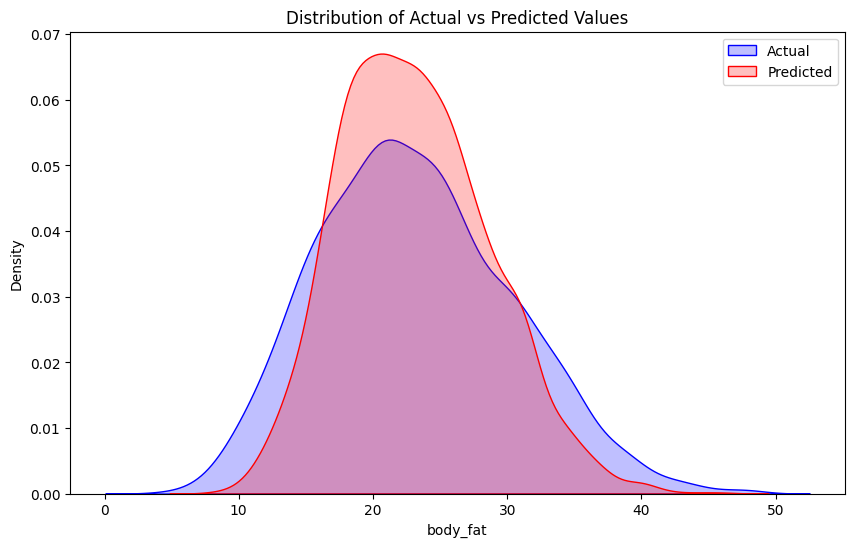
\includegraphics[width=0.8\linewidth]{graphics/dis_ac_vs_pre.png}
    \caption{Biểu đồ phân bố mật độ}
\end{figure}

\textbf{Phân phối tương đối giống nhau:} Cả hai đường cong của giá trị thực tế và dự đoán đều có hình dạng tương tự nhau, cho thấy mô hình đã bắt được xu hướng chung của dữ liệu.

\textbf{Mô hình có xu hướng dự đoán hơi thấp:} Đỉnh của đường cong dự đoán có vẻ hơi dịch chuyển về phía bên trái so với đỉnh của đường cong thực tế, cho thấy mô hình có xu hướng dự đoán giá trị phần trăm mỡ cơ thể hơi thấp so với giá trị thực tế.

Dựa trên biểu đồ này, có thể kết luận rằng mô hình hồi quy tuyến tính đã thực hiện khá tốt trong việc dự đoán lượng mỡ cơ thể. Tuy nhiên, vẫn còn một số không chính xác nhất định, đặc biệt là mô hình có xu hướng đánh giá thấp lượng mỡ cơ thể.

\newpage

\begin{figure} [!htp]
    \centering
    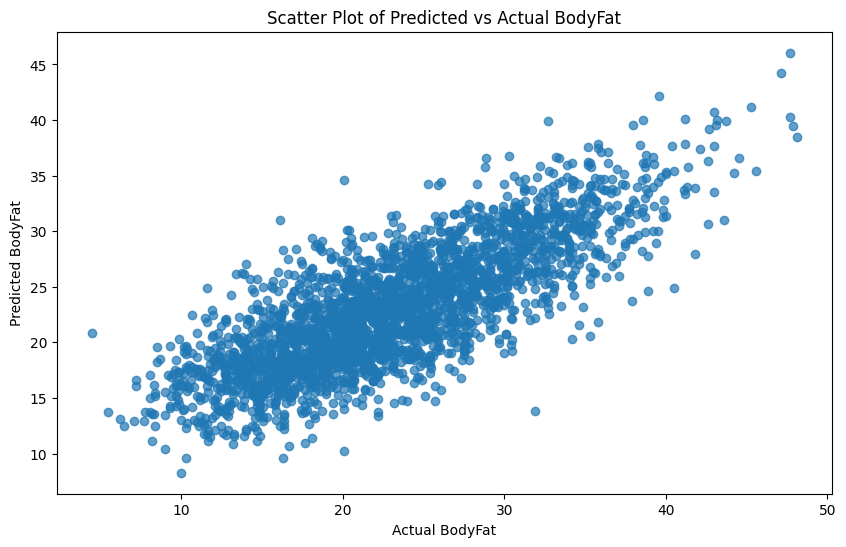
\includegraphics[width=0.8\linewidth]{graphics/scatt_pre_vs_ac.png}
    \caption{Biểu đồ phân tán}
\end{figure}

\textbf{Mối quan hệ tuyến tính:} Các điểm dữ liệu có xu hướng phân bố theo một đường thẳng, cho thấy có mối quan hệ tuyến tính giữa giá trị dự đoán và giá trị thực tế.

\textbf{Độ chính xác:} Phần lớn các điểm dữ liệu nằm gần đường thẳng y=x, cho thấy mô hình dự đoán khá chính xác. Tuy nhiên, vẫn có một số điểm dữ liệu nằm xa đường thẳng này, đặc biệt ở vùng giá trị thực tế lớn hơn 40.

\textbf{Các điểm ngoại lệ:} Có một số điểm dữ liệu nằm khá xa các điểm khác, đặc biệt ở vùng giá trị thực tế nhỏ hơn 15 và lớn hơn 45.

Biểu đồ phân tán này cho thấy mô hình hồi quy tuyến tính đã xây dựng được một mối quan hệ tuyến tính khá tốt giữa các biến độc lập và biến phụ thuộc.

Từ những đánh giá sơ bộ trên có thể kết luận rằng mô hình Linear Regression phù hợp với bài toán dự đoán tỷ lệ mỡ trên cơ thể. Thử nghiệm mô hình trên giá trị giả định: \textbf{25 tuổi}, \textbf{giới tính nam}, \textbf{chiều cao 166 cm}, và \textbf{cân nặng 77.7 kí} cho kết quả như sau:

\newpage

\begin{figure} [!htp]
    \centering
    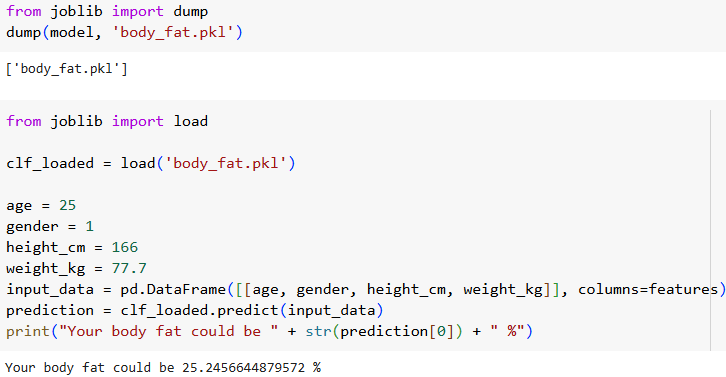
\includegraphics[width=0.9\linewidth]{graphics/result_bf.png}
    \caption{Kết quả dự đoán phần trăm mỡ dựa trên dữ liệu đầu vào giả định}
\end{figure}

\subsubsection{Đo độ thăng bằng của cơ thể}

Chức năng này sử dụng MediaPipe và OpenCV để theo dõi tư thế người dùng qua camera, thu thập mẫu chuẩn và đo độ thăng bằng dựa trên vị trí tâm khối (COM).

\newpage
\begin{figure}[!htp]
    \centering
    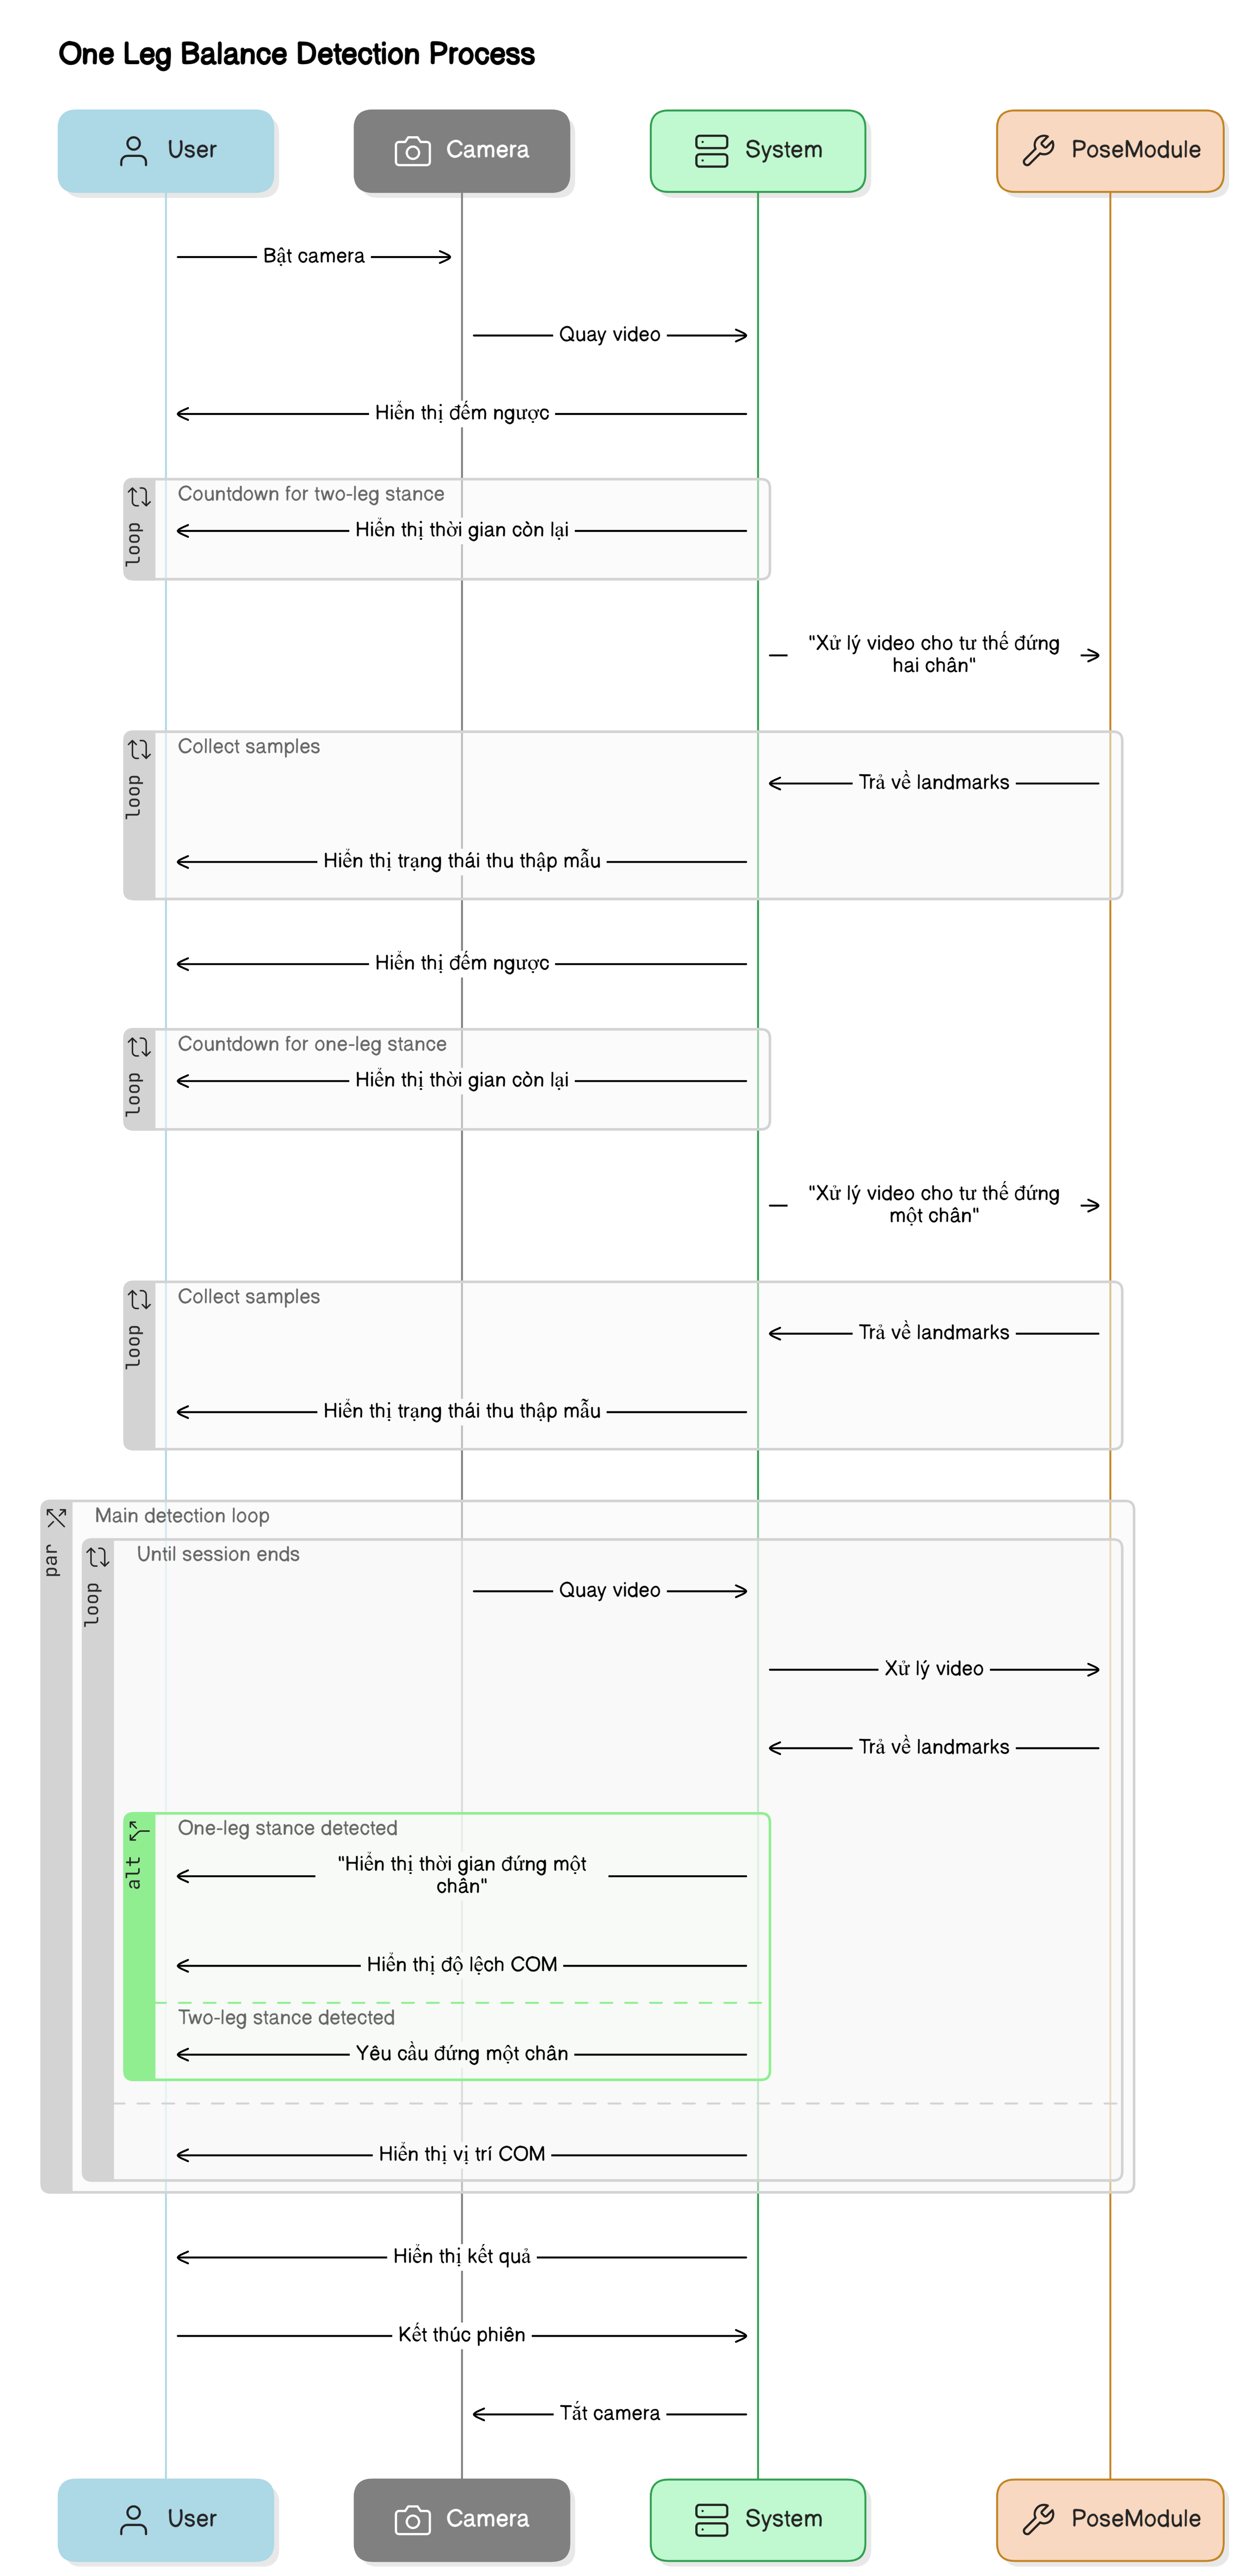
\includegraphics[width=0.6\linewidth]{graphics/oneleg_chart.png}
    \caption{Quá trình nhận diện thời gian thăng bằng 1 chân}
\end{figure}
\newpage

\paragraph{Kiến trúc và luồng hoạt động}
\begin{itemize}
  \item \textbf{Giai đoạn thu thập mẫu chuẩn:} Người dùng đứng hai chân để thu thập mẫu \texttt{two\_legs\_samples}, sau đó đứng một chân để thu thập mẫu \texttt{one\_leg\_samples}. Mỗi mẫu là một vector tọa độ landmarks.
  \item \textbf{Giai đoạn đo đạc chính:} Xử lý video liên tục, xác định tư thế hiện tại qua cosine similarity giữa vector hiện tại và hai bộ mẫu. Khi phát hiện tư thế một chân, ghi nhận thời gian và độ lệch COM.
  \item \textbf{Giai đoạn kết thúc:} Khi người dùng trở về tư thế hai chân, tính tổng thời gian đứng một chân và độ lệch trung bình, trả về kết quả.
\end{itemize}

\paragraph{Phân tích chi tiết các thành phần}

\subparagraph{Xử lý video và hiển thị}
\begin{itemize}
  \item Sử dụng \texttt{cv2.VideoCapture} để lấy khung hình, \texttt{cv2.putText}, \texttt{cv2.circle}, \texttt{cv2.imshow} để vẽ hướng dẫn và kết quả.
  \item Hàm \texttt{countdown(cap, duration, message)}: vòng lặp dựa trên \texttt{time.time()}, cập nhật thời gian còn lại và hiển thị đếm ngược, cho phép thoát sớm bằng phím \texttt{q}.
\end{itemize}

\subparagraph{Trích xuất và chuyển đổi landmarks}
\begin{itemize}
  \item Khởi tạo \texttt{mp\_pose.Pose} với \texttt{min\_detection\_confidence=0.5} và \texttt{min\_tracking\_confidence=0.5}.
  \item \texttt{landmarks\_to\_vector(landmarks)}: chuyển danh sách landmarks thành vector NumPy 1 chiều chứa \texttt{[x\_1, y\_1, x\_2, y\_2, \dots]}.
\end{itemize}

\subparagraph{Đo độ tương đồng giữa các mẫu}
\begin{itemize}
  \item \texttt{calculate\_max\_similarity(current\_vector, samples)}: lặp qua các mẫu, tính cosine similarity bằng \texttt{1 - cosine(v1, v2)}, chọn giá trị cao nhất để quyết định tư thế.
\end{itemize}

\subparagraph{Thu thập mẫu}
\begin{itemize}
  \item \texttt{collect\_samples(pose, cap, num\_samples, instruction\_text)}: thu thập \texttt{num\_samples} vector landmarks trong tối đa 30 giây, chờ 1 giây giữa mỗi mẫu, hiển thị số lượng mẫu đã thu.
\end{itemize}

\subparagraph{Phân tích phiên “đứng một chân”}
\begin{itemize}
  \item \texttt{one\_leg\_balance\_detection(camera\_index, num\_samples)}:
    \begin{enumerate}
      \item Đếm ngược chuẩn bị, thu hai bộ mẫu (hai chân và một chân).
      \item Với mỗi khung hình, ước tính COM qua trung điểm hông trái – hông phải, quy đổi sang pixel.
      \item Tính cosine similarity với hai bộ mẫu, xác định tư thế.
      \item Khi ở tư thế một chân, bắt đầu phiên, tính offset theo trục \(x\) giữa COM hiện tại và COM baseline, lưu vào \texttt{session\_offsets}.
      \item Khi quay về hai chân, kết thúc phiên, tính \(\text{session\_duration}\) và \(\text{avg\_offset}\), trả về kết quả.
    \end{enumerate}
\end{itemize}

\paragraph{Ưu điểm và hướng cải thiện}

\subparagraph{Ưu điểm}
\begin{itemize}
  \item Giao diện trực quan: đếm ngược, hướng dẫn và kết quả thời gian thực.
  \item Sử dụng cosine similarity hiệu quả để phân loại tư thế.
  \item Quy trình rõ ràng, dễ bảo trì.
\end{itemize}

\subparagraph{Hạn chế và cải thiện}
\begin{itemize}
  \item Ứng dụng COM chỉ dựa trên trung điểm hông có thể thiếu chính xác; có thể bổ sung các điểm khác như vai, đầu gối.
  \item Cần xử lý nhiễu từ landmarks (ánh sáng, góc quay) bằng bộ lọc hoặc smoothing.
  \item Thay vì \texttt{time.sleep(1)}, có thể sampling linh hoạt dựa trên thay đổi thực tế của landmarks.
\end{itemize}

\paragraph{Kết luận}

Giải pháp cho phép đo độ thăng bằng dựa trên phân tích COM từ MediaPipe, với quy trình thu thập mẫu và đo đạc rõ ràng. Tuy còn một số hạn chế về độ chính xác và hiệu suất, khung sườn hiện tại là nền tảng vững chắc cho các cải tiến sau này.


\subsubsection{Đưa ra các đánh giá và lời khuyên dựa trên các chỉ số của cơ thể}
Sau khi nội suy và dự đoán các thông số sức khoẻ của cơ thể, sử dụng \href{https://aistudio.google.com/u/0/apikey}{API của mô hình Google Gemini Pro 1.5 Flash} để đưa ra các đánh giá và lời khuyên để cải thiện sức khoẻ người dùng.

\begin{figure} [!htp]
    \centering
    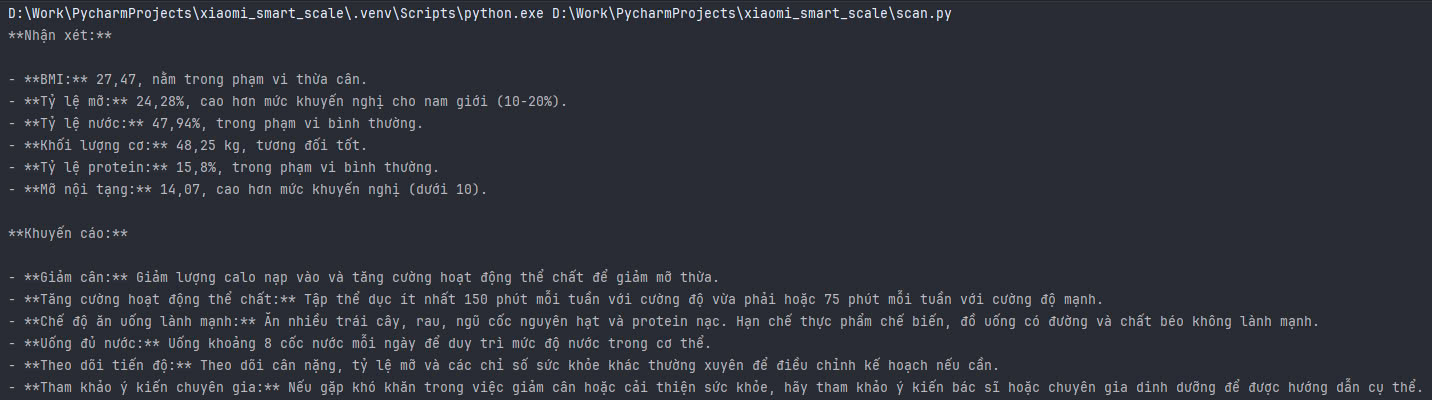
\includegraphics[width=1\linewidth]{graphics/ai_rcmd.jpg}
    \caption{Sử dụng AI để đánh giá và đưa ra các lời khuyên về sức khoẻ của người dùng}
\end{figure}

\subsubsection{Đọc các đánh giá và lời khuyên cho người dùng}
Sau nhận các đánh giá từ AI, sử dụng \href{https://pypi.org/project/gTTS/}{thư viện gTTS (Google Text-to-Speech)} để đọc các đánh giá cho người dùng

\begin{lstlisting}[language=python,caption={Sử dụng thư viện gTTS để đọc các đánh giá của AI}]
from gtts import gTTS
import os

def read_recommend_vietnamese(user_info, text):

    tts = gTTS(text = text, lang = 'vi', slow=False)

    tts.save("audio/audio.mp3")

    os.system("start audio/audio.mp3")  # Windows
\end{lstlisting}

\subsection{Đánh giá các số liệu nội suy và dự đoán bởi AI so với thiết bị có cảm biến}
Để đánh giá các chỉ số cơ thể từ nội suy theo công thức và dự đoán bằng trí tuệ nhân tạo, em sử dụng cân điện tử \textbf{Xiaomi Smart Scale 2} để lấy cân nặng ban đầu và tiến hành tính toán, dự đoán ra các thông số cơ thể so sánh với thiết bị cân điện tử có cảm biến \textbf{(Xiaomi Scale Composition S400)} thu được bảng sau:

\begin{table}[!htp]
\centering
\begin{tabular}{clccr}
\toprule
STT & Chỉ số & Xiaomi Smart Scale 2 & Xiaomi Scale Composition S400 & Sai số \\
\midrule
1 & Cân nặng & 75.55 & 75.6 & 0.07\% \\
2 & BMI & 27.42 & 27.4 & 0.07\% \\
3 & BMR & 1755.21 & 1599 & 9.77\% \\
4 & TDEE & 2720.58 & None &  None\\
5 & LBM & 51.58 & 56.8 & 9.19\% \\
6 & Phần trăm mỡ (AI) & 24.21 & 24.8 & 2.38\% \\
8 & Phần trăm nước & 47.99 & 52.5 & 8.59\% \\
9 & Khối lượng xương & 2.58 & 2.9 & 11.03\% \\
10 & Khối lượng cơ & 48.2 & 53.9 & 10.58\% \\
11 & Phần trăm protein & 15.81 & 18 & 12.17\% \\
12 & Mỡ nội tạng & 14 & 10 & 40.00\% \\
13 & Cân nặng lý tưởng & 60.2 & 60.2 & 0.00\% \\
\bottomrule
\end{tabular}
\caption{So sánh chỉ số giữa các thông số tính toán và Xiaomi Scale Composition S400}
\end{table}

Bảng so sánh trên cung cấp một cái nhìn chi tiết về sự khác biệt giữa các thông số nội suy theo công thức, dự đoán bằng AI và Xiaomi Scale Composition S400. Cả hai đều thể hiện được các chỉ số cơ thể cơ bản như cân nặng, BMI, nhưng S400 cung cấp nhiều thông tin chi tiết hơn về thành phần cơ thể.

Nhìn chung, các chỉ số đo được từ S400 có sự chênh lệch không đáng kể so với các thông số nội suy và dự đoán, ngoại trừ một số chỉ số như mỡ nội tạng có sự chênh lệch khá lớn (40\%).

Tuy nhiên, có một số lưu ý như:

\begin{itemize}
    \item \textbf{Sai số:} Mặc dù S400 cho kết quả chi tiết hơn, nhưng vẫn tồn tại sai số nhất định ở một số chỉ số. Do đó, không nên quá phụ thuộc vào một lần đo mà nên theo dõi kết quả trong một thời gian dài để có cái nhìn tổng quan chính xác hơn.
    \item \textbf{Giá thành:} Thông thường, các mẫu cân có nhiều tính năng hơn sẽ có giá thành cao hơn. Vì vậy, S400 có thể có giá thành cao hơn so với một chiếc cân điện tử thông thường được áp dụng các công thức nội suy và dự đoán của AI.
\end{itemize}

\subsection{Lưu trữ thông tin người dùng}
Những thông tin cơ bản của người dùng và các chỉ số đo, tính toán được sẽ được lưu lại dưới dạng 1 file .csv để có thể trực quan hoá và phục vụ cho mục đích nghiên cứu sau này, file .csv lưu lại các thông tin sau: \textbf{datetime, name, age, gender, height, weight, dob, activity\_factor, bmi, bmr, tdee, lean\_body\_mass, fat\_percentage, water\_percentage, bone\_mass, muscle\_mass, protein\_percentage, visceral\_fat, ideal\_weight}

\begin{figure}[!htp]
    \centering
    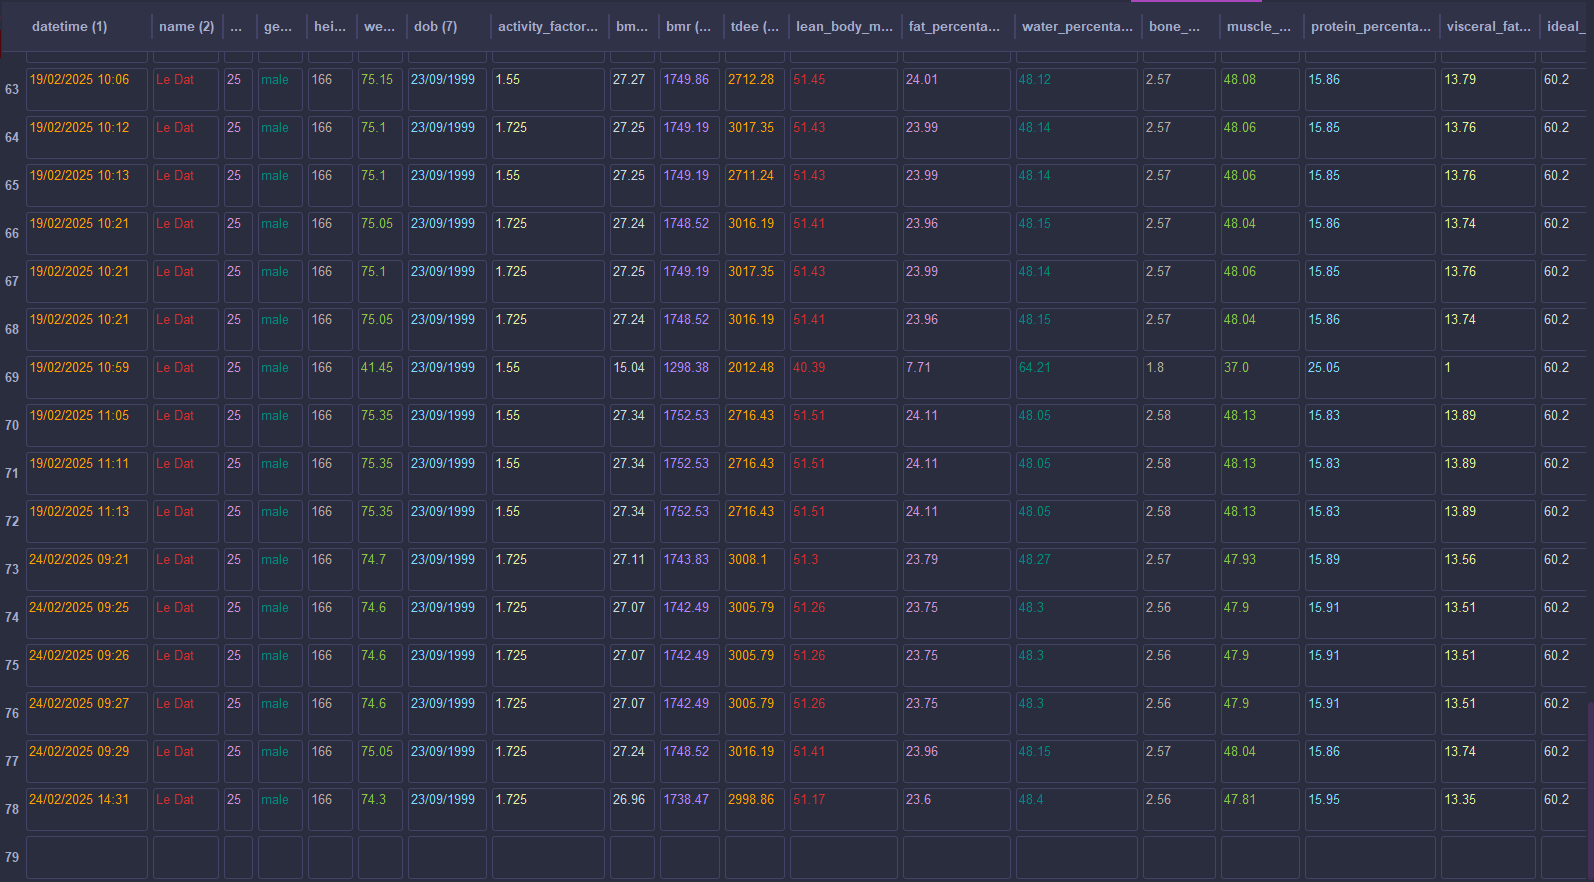
\includegraphics[width=0.7\linewidth]{graphics/csv.png}
    \caption{Các thông tin của người dùng được lưu trữ trong file csv}
\end{figure}

\subsection{Trực quan hóa dữ liệu sức khỏe thông qua CoreIoT}
\subsubsection{Cấu hình thiết bị trên nền tảng IoT}
Trên nền tảng CoreIoT, việc cấu hình thiết bị là bước quan trọng nhằm trực quan hóa các thông số sức khỏe, cho phép Gateway giao tiếp hiệu quả với nền tảng thông qua giao thức MQTT. Để thực hiện, người dùng cần truy cập vào thẻ \textbf{Entities}, sau đó chọn thẻ con \textbf{Devices} để thiết lập kết nối và truyền dữ liệu từ thiết bị IoT.

\begin{figure}[!htp]
    \centering
    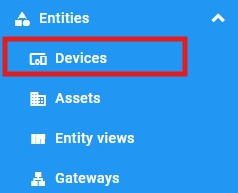
\includegraphics[width=0.5\linewidth]{graphics/coreiot_device.png}
    \caption{Chọn thẻ Devices để cấu hình thiết bị giao tiếp với nền tảng CoreIoT}
    \label{fig:coreiot-device}
\end{figure}
\newpage

Trong phần \textbf{Device Credentials}, người dùng cần thiết lập phương thức xác thực cho thiết bị. Nền tảng CoreIoT hỗ trợ nhiều tùy chọn xác thực, bao gồm \textbf{Access token}, \textbf{X.509}, và \textbf{MQTT Basic}. Trong dự án này, phương thức \textbf{MQTT Basic} được sử dụng, tận dụng các thông tin như \textbf{ClientID}, \textbf{User Name}, và \textbf{Password} để đảm bảo thiết bị kết nối an toàn và ổn định với nền tảng.

\begin{figure}[!htp]
    \centering
    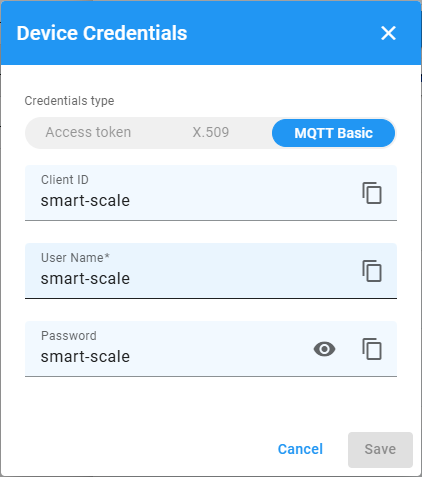
\includegraphics[width=0.5\linewidth]{graphics/coreiot_mqtt.png}
    \caption{Cấu hình Device Credentials trên nền tảng CoreIoT}
    \label{fig:device-credentials}
\end{figure}

Sau khi hoàn tất việc thiết lập thông tin xác thực trong thẻ \textbf{Device Credentials}, các thông tin này sẽ được sử dụng để cấu hình trong mã nguồn của thiết bị. Quy trình này đảm bảo thiết bị giao tiếp chính xác với nền tảng CoreIoT.

\begin{figure}[!htp]
    \centering
    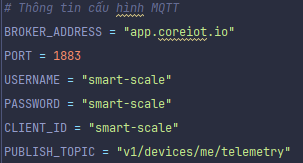
\includegraphics[width=0.5\linewidth]{graphics/mqtt_info.png}
    \caption{Cấu hình các thông số xác thực MQTT trong mã nguồn của thiết bị}
    \label{fig:mqtt-config}
\end{figure}

Để truyền các giá trị thông số sức khỏe từ thiết bị lên nền tảng CoreIoT, đoạn mã sau được sử dụng:

\begin{lstlisting}[language=python,caption={Gửi dữ liệu sức khỏe lên CoreIoT qua MQTT}]
mqtt_client.publish(PUBLISH_TOPIC, health_data.get_body_composition())
\end{lstlisting}

Trong đó, \textbf{PUBLISH\_TOPIC = "v1/devices/me/telemetry"} là topic mặc định mà nền tảng CoreIoT sử dụng để nhận dữ liệu từ thiết bị.

Cuối cùng, để kiểm tra và quan sát các giá trị thông số sức khỏe đã được cập nhật, người dùng có thể chuyển sang thẻ \textbf{Latest telemetry} của thiết bị trên giao diện CoreIoT.

\begin{figure}[!htp]
    \centering
    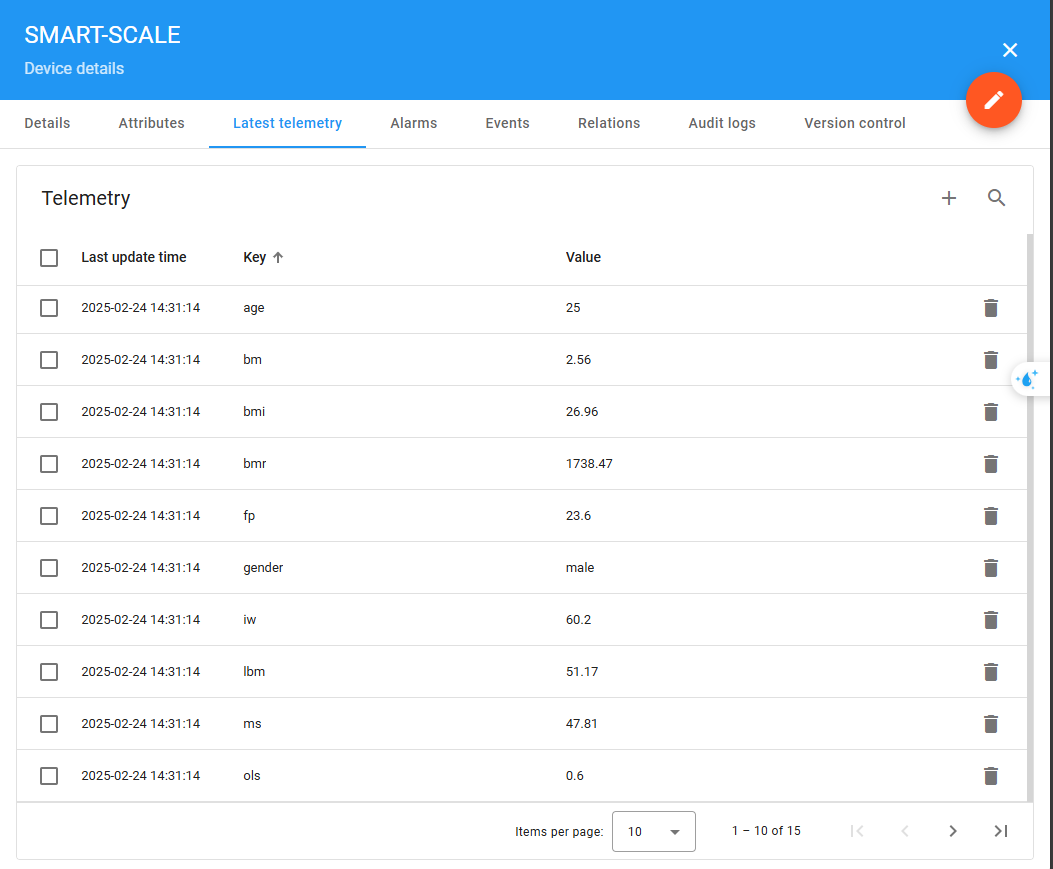
\includegraphics[width=0.8\linewidth]{graphics/lastest_telemetry.png}
    \caption{Các giá trị thông số sức khỏe được cập nhật trong thẻ Latest telemetry của thiết bị}
    \label{fig:latest-telemetry}
\end{figure}

\newpage

\subsubsection{Cài đặt bảng điều khiển để hiển thị các thông số sức khỏe}

Sau khi các thông số sức khỏe từ cân điện tử thông minh đã được truyền tải và hiển thị trong thẻ \textbf{Latest telemetry} của thiết bị trên giao diện CoreIoT, bước tiếp theo là chuyển sang thẻ \textbf{Dashboard} để cấu hình và trực quan hóa các thông số này trên bảng điều khiển chính.

\begin{figure}[!htp]
    \centering
    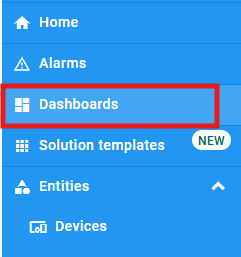
\includegraphics[width=0.5\linewidth]{graphics/dashboard.png}
    \caption{Thẻ Dashboard trên giao diện của nền tảng CoreIoT}
    \label{fig:dashboard-tab}
\end{figure}

\newpage

Tiếp theo, người dùng cần tạo một Dashboard mới và đặt tên cho nó để dễ dàng quản lý và nhận diện.

\begin{figure}[!htp]
    \centering
    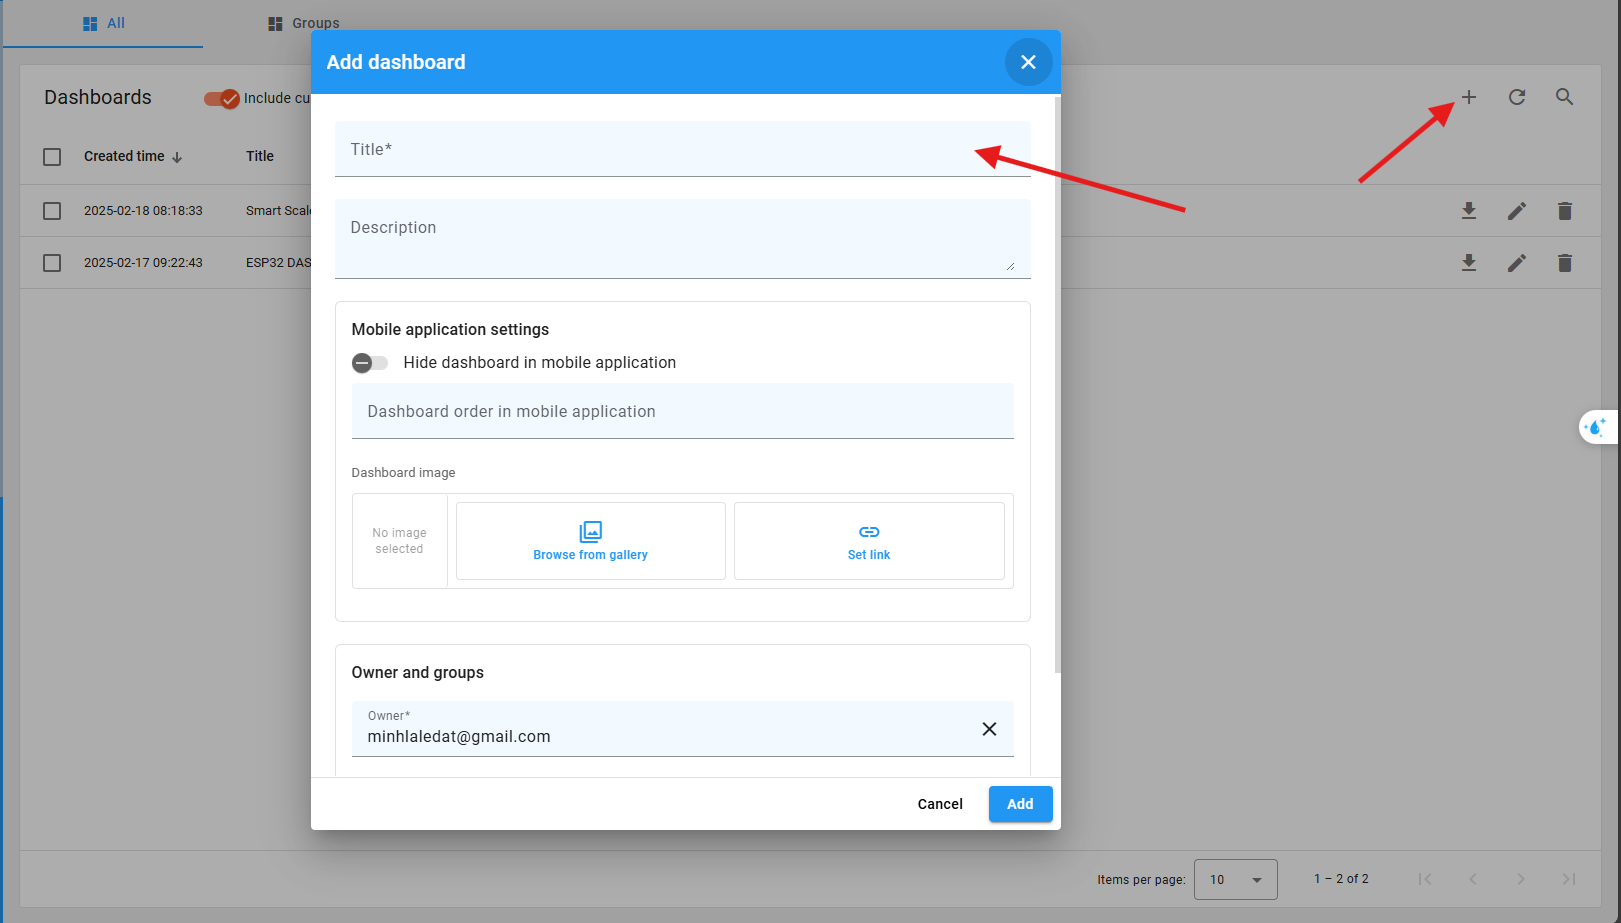
\includegraphics[width=0.9\linewidth]{graphics/create_named_dashboard.png}
    \caption{Tạo và đặt tên cho Dashboard mới}
    \label{fig:create-dashboard}
\end{figure}

Sau khi Dashboard được tạo, người dùng có thể thêm các phần tử (widgets) để hiển thị trực quan các thông số sức khỏe, giúp theo dõi dữ liệu một cách hiệu quả.

\begin{figure}[!htp]
    \centering
    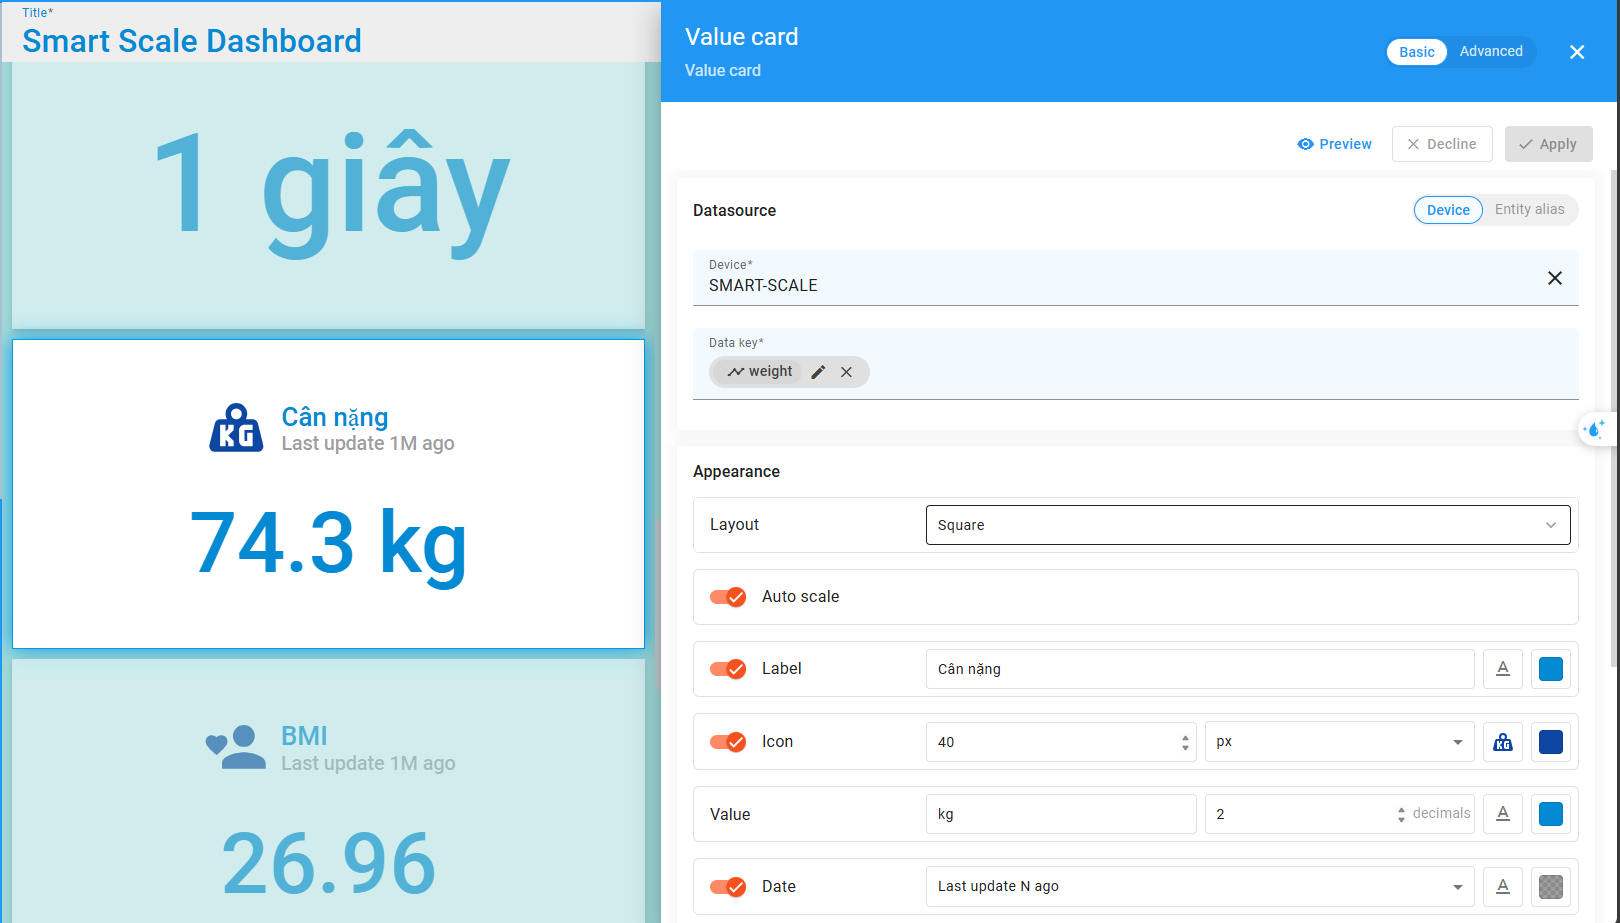
\includegraphics[width=0.75\linewidth]{graphics/init_element_dashboard.png}
    \caption{Cấu hình các thông số cho phần tử hiển thị trên Dashboard}
    \label{fig:config-widget}
\end{figure}

\newpage

Trong quá trình cấu hình phần tử, người dùng cần cung cấp các thông tin sau:

\begin{itemize}
    \item \textbf{Device:} Tên của thiết bị đã được thiết lập trước đó trong mục \textbf{Entities} > \textbf{Devices}.
    \item \textbf{Data key:} Giá trị tương ứng với thông số sức khỏe được truyền từ Gateway, có thể tra cứu trong thẻ \textbf{Latest telemetry}.
\end{itemize}

Ngoài ra, nền tảng CoreIoT còn cung cấp các tùy chọn tinh chỉnh như màu sắc, kích thước và kiểu hiển thị của các phần tử trên Dashboard, cho phép người dùng điều chỉnh giao diện theo nhu cầu cụ thể.

\begin{figure}[!htp]
    \centering
    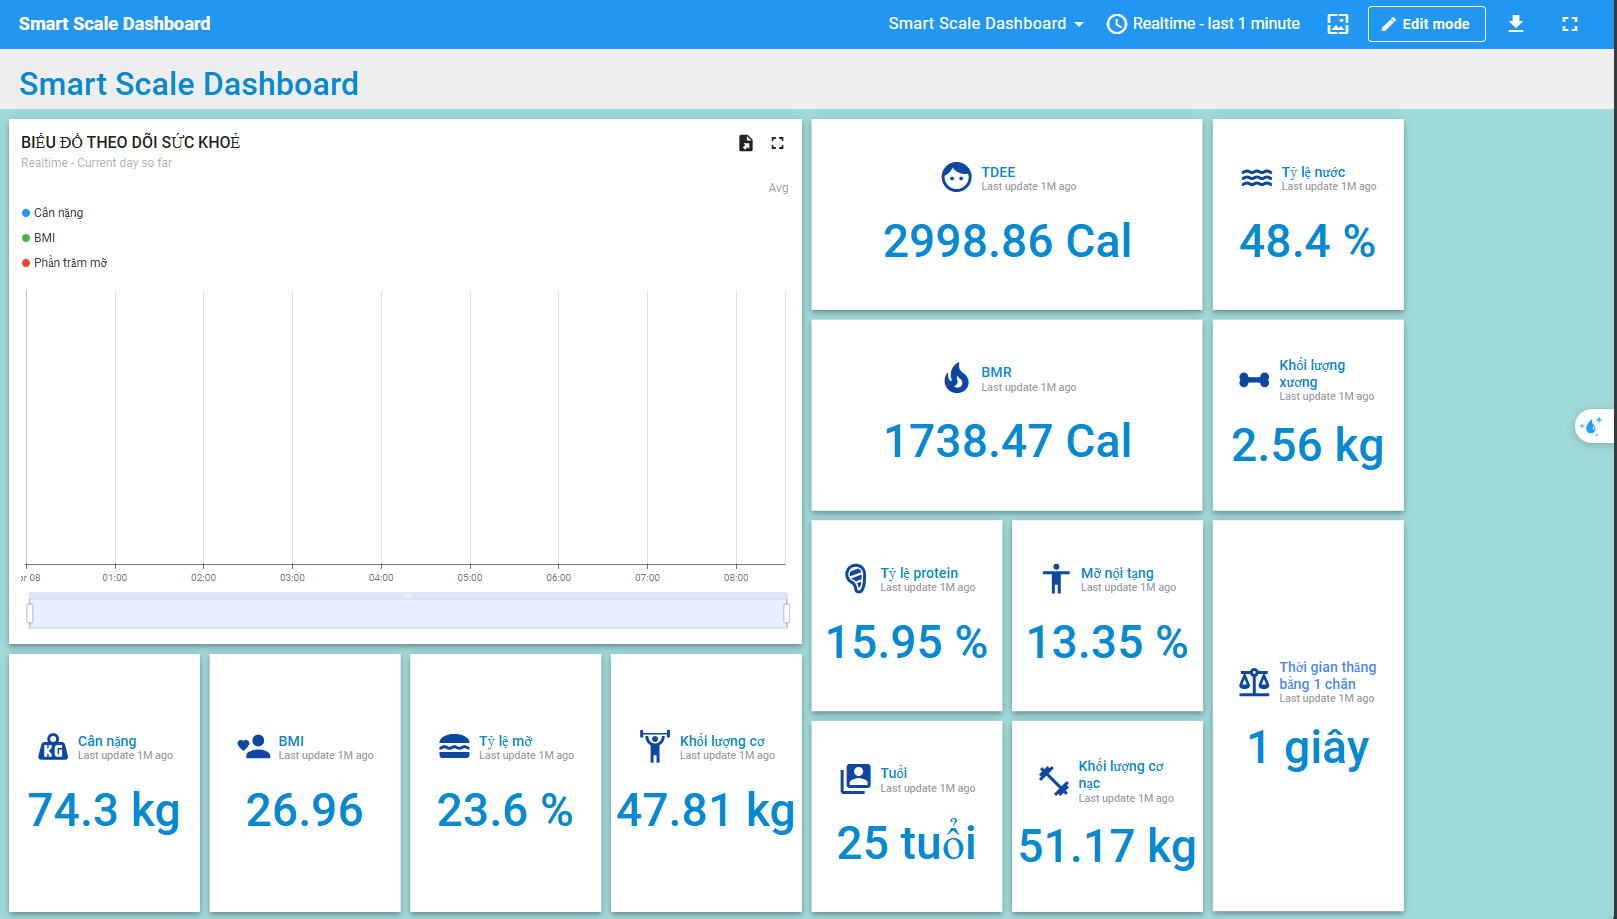
\includegraphics[width=0.75\linewidth]{graphics/final_dashboard.png}
    \caption{Dashboard của dự án sau khi được tinh chỉnh và hoàn thiện}
    \label{fig:final-dashboard}
\end{figure}